{~ }

{
\includegraphics{images/image06.png}}

\subsection{\texorpdfstring{{\protect
\includegraphics{images/image06.png}}{~}}{~}}\label{h.z6ne0og04bp5}

{
\includegraphics{images/image02.jpg}}

{OBD Testing and Tool Documentation}

{XX.XX.2016}

{─}

{Zoran Prodanovic \& Zlatan Zaric}

{Technische Universität Graz - Institut für Technische Informatik}

{Inffeldgasse 16 }

{8010 Graz}

{Table of Contents}

{}

{\protect\hyperlink{h.w1vd037gtz71}{Abstract}}

{\protect\hyperlink{h.ca2gtl63cpbb}{Motivation}}

{\protect\hyperlink{h.ku3zfbnqma3q}{Market Analysis of Existing OBD
Tools}}

{\protect\hyperlink{h.6vg54mt7ey8d}{Windows}}

{\protect\hyperlink{h.plxr4kgyruuo}{Ubuntu}}

{\protect\hyperlink{h.e4qn0u5p3hu9}{Conclusion}}

{\protect\hyperlink{h.lzjv4pe0xkgv}{Goals}}

{\protect\hyperlink{h.4p7xi5bvhxdr}{Specifications}}

{\protect\hyperlink{h.56kfpodyq5td}{Non Technical Specifications}}

{\protect\hyperlink{h.m62hdjh1p5au}{The On-Board-Diagnostic Basics}}

{\protect\hyperlink{h.a007s3g11xnb}{Busses}}

{\protect\hyperlink{h.g52kpz9o7mut}{Universal Serial Bus (USB)}}

{\protect\hyperlink{h.sndep0jf1bfd}{The 4 Transfer Types}}

{\protect\hyperlink{h.90a05v4yh1c6}{Control Transfers}}

{\protect\hyperlink{h.nxp3faj0xgfy}{Interrupt Transfers}}

{\protect\hyperlink{h.icibxq66s779}{Isochronous Transfers}}

{\protect\hyperlink{h.3yadg7wz9shv}{Bulk Transfers}}

{\protect\hyperlink{h.c8rxmh3196o7}{Descriptors}}

{\protect\hyperlink{h.1mpv5d9ppg1r}{Device Descriptor}}

{\protect\hyperlink{h.73p9cggljvzi}{Configuration Descriptor}}

{\protect\hyperlink{h.6og933fa49b9}{Interface Descriptor}}

{\protect\hyperlink{h.v1p4ngh8b7ot}{Endpoint ~Descriptor}}

{\protect\hyperlink{h.tyeikwcmymv0}{String ~Descriptor}}

{\protect\hyperlink{h.n9ec73ci5cit}{Requests}}

{\protect\hyperlink{h.sukmqmhc4ldi}{Command Structure and Behaviour}}

{\protect\hyperlink{h.4dw71h9dkw49}{Service Modes
(http://www.outilsobdfacile.com/obd-mode-pid.php)}}

{\protect\hyperlink{h.zg0lajxcv3vk}{Parameter Identifier}}

{\protect\hyperlink{h.k3ecyfg5l7ib}{Implementation}}

{\protect\hyperlink{h.o5tk1rwy6zuu}{Serial Communication}}

{\protect\hyperlink{h.8ukx9pv2y8wv}{Serial Communication}}

{\protect\hyperlink{h.nfl0zlavkqps}{Emulation}}

{\protect\hyperlink{h.rpls244qrcic}{Databases}}

{\protect\hyperlink{h.fbh3ldin73fx}{OBD Base}}

{\protect\hyperlink{h.tbf8n411o12j}{Calculation Values}}

{\protect\hyperlink{h.t1w3v8o28dma}{Value Mapping Values}}

{\protect\hyperlink{h.nvvniy6ibvmm}{Bit Mapping Values}}

{\protect\hyperlink{h.v3wlh8gjmo1s}{Bit Combination Mapping Values}}

{\protect\hyperlink{h.q2wfq2ktke27}{Inner Workings}}

{\protect\hyperlink{h.wbiklph9gdnl}{ELM Commands}}

{\protect\hyperlink{h.8c6emwe3lhuv}{Configuration}}

{\protect\hyperlink{h.upb9og5wn4q0}{Project Specific Implementation}}

{\protect\hyperlink{h.dfu1gktb8xw}{OBDCU}}

{\protect\hyperlink{h.pxkpe4k3lbn1}{Installation How To}}

{\protect\hyperlink{h.agltrea2kef8}{vhci\_hcd}}

{\protect\hyperlink{h.8woybtsjfs8s}{libusb\_vhci (userspace tools):}}

{\protect\hyperlink{h.73mzfu9s6v0d}{Building the Project}}

{\protect\hyperlink{h.totk00jqaso2}{Software Development Techniques}}

{\protect\hyperlink{h.qmc1u1ly9e76}{Basics}}

{\protect\hyperlink{h.al3idr34x902}{Extreme Programming}}

{\protect\hyperlink{h.98eiyanf314e}{Automotive SPICE}}

{\protect\hyperlink{h.mifm7q3zf07v}{Clean Code}}

{\protect\hyperlink{h.8nawqkcgevsc}{Realization}}

{\protect\hyperlink{h.xkuwr51j6zad}{Conclusion}}

{\protect\hyperlink{h.mzh64o82gvdq}{References}}

\hypertarget{h.w1vd037gtz71}{\section{\texorpdfstring{{Abstract}}{Abstract}}\label{h.w1vd037gtz71}}

{TBD after feedback}\textsuperscript{\protect\hyperlink{cmnt1}{{[}a{]}}}

\hypertarget{h.ca2gtl63cpbb}{\section{\texorpdfstring{{Motivation}}{Motivation}}\label{h.ca2gtl63cpbb}}

{The motivation for this project is the increasing complexity of modern
car systems. The amount of integrated control units in automotive
systems these days tends to go beyond 80. The resulting energy
consumption for the electrical components in such a system sums up to
2,5 kW. This grounds the decision of the automotive industry to deal
with }{its }{own energy management of these components. Considering the
number of control units and their energy consumption an effective
handling of these units }{seems inevitable}{. Since the knowledge about
the fundamental functionality of control units is kept with the
manufacturer, serious knowledge deficit surfaces regarding control units
from the perspective of a common service mechanic. Thus leading to a
dependency on expensive information and/or tools provided by the
manufacturer of the automobile.}

{The car service shop is forced to rely on those tools. If suspicion of
a fault in a control unit arises it is common practice to change the
whole unit to resolve this suspicion rather than fixing the real cause
of the actual error.}

{On the other hand this opens possibilities for the manufacturer to keep
his income over development periods high. Since knowledge about the
specifics or the right protocols is restricted communication with the
full functionality extent giving}{~automotive manufacturers the chance
to sell those protocols or a service for diagnosing, keeping their
income high.}

{After discovering that there are standards defining most of the
diagnostic trouble codes (DTCs) and the possibility to request those
with hardware available at an economic
price}\textsuperscript{\protect\hyperlink{ftnt1}{{[}1{]}}}{~it seems
reasonable to develop an open source software implementing those
functio}{n}{alities. Further than just requesting DTCs the software is
meant to entail ELM327 features as well. }

\hypertarget{h.ku3zfbnqma3q}{\subsection{\texorpdfstring{{Market
Analysis of Existing OBD
Tools}}{Market Analysis of Existing OBD Tools}}\label{h.ku3zfbnqma3q}}

{}

{The first impression of the OBD diagnostic tools market may seem vast,
but focusing on open source solutions it is limited to a handful of
tools.}

{During the research phase we found different software starting by pyOBD
and ScanTool, over ScanMaster and EasyObd up to OBD Auto Doctor. When
putting them under practical tests huge difficulties emerged. The
following analysis is meant to provide the foundation for this bachelor
thesis to implement an open source OBD tool as well as a test system for
OBD tools under Linux, which should easily be }{extendable }{to
Windows.}

{}

{The strategy on keeping the software easily extendable is to adapt the
general programming style to use system independent libraries, thus
ensuring the ability to run on most common systems. }{As}{~a foundation
}{of the market analysis }{testing the currently available software seem
reasonable. Therefore the }{basic testing strategy is to choose a
distribution and try to execute the following steps:}

{}

\begin{enumerate}
\tightlist
\item
  {establish a connection to the OBD interface via an ELM327
  microcontroller }
\item
  {read trouble codes produced by self-made errors}
\item
  {reset trouble code memory}
\end{enumerate}

{}

{Those steps define the basic functionalities in every OBD standard
which can be considered as the minimum requirements for an OBD diagnosis
tool.}

{By acquiring two standard USB to OBD cables at least hardware
independence can be established to a certain degree. Additionally the
conclusion, that the costs of the required hardware are low, can be
drawn and thus leading to average consumers with low budgets
representing the target audience. Due to the requirement of hardware
independence the focus of the project shifts to a pure software
implementation. Even though only the use of hardware based on the ELM327
chip is intended, compatibility for most ELM chips is the long term
goal. }

{Taking the variety of the target audience into account, as many
different cars and systems }{as available }{served as testing
environments to experience the behaviour of the tested tools under
different circumstances. Those cars consist of a Renault Trafic 2006 1.9
TDI, an Opel Vivaro 2009, an Opel Zafira 2004 as well as a VW Sharan
2003 1.9 TDI. By using Windows and Ubuntu the majority of
}{distributions }{are covered.}

\hypertarget{h.6vg54mt7ey8d}{\subsubsection{\texorpdfstring{{Windows}}{Windows}}\label{h.6vg54mt7ey8d}}

{F}{our different OBD softwares on a Windows 7 OS are tested:}

\begin{itemize}
\tightlist
\item
  {EasyObdII Version 2.5}
\item
  {OBD Auto Doctor}
\item
  {ScanMaster-ELM DEMO}
\item
  {OBD 2007}
\end{itemize}

{}

{With OBD 2007 and EasyObdII Version 2.5 problems occurred while just
trying to connect to the control unit, making it difficult to conduct
the tests. Different attempts to solve this problem failed.}

{Since only trial/demo versions are available for free, the range of
testable functions is limited to measuring the actual engine RPM, the
vehicle speed or the load value.}{~}{Due to the encountered problems, a
satisfying analysis could not be executed thoroughly.}

\hypertarget{h.plxr4kgyruuo}{\subsubsection{\texorpdfstring{{Ubuntu}}{Ubuntu}}\label{h.plxr4kgyruuo}}

{Connecting to the control unit under Linux proved to be a problem as
the ELM327 uses the USB port (ttyUSB\#) but most of the tested software
only searches for COM ports (ttyS\#).}

{Assuming intact hardware, no immediate solution appeared of how to
mount the USB device onto the COM port nor how to configure the software
such that it connects to the USB port. }{However, }{using the low level
standard software }{s}{creen supplied by Linux seemed to be the best
approach, as it enables communication with any serial device in form of
HEX commands. With this approach the request for trouble codes in HEX
format is possible, but additional information such as datasheets,
computer knowledge as well as forums for decoding the response are
necessary.}

{}

\hypertarget{h.e4qn0u5p3hu9}{\subsubsection{\texorpdfstring{{Conclusion}}{Conclusion}}\label{h.e4qn0u5p3hu9}}

{Although spending much}{~time in trying to enable the software's
functionality on both systems, the benefit is limited. Judging from the
interface of those freeware tools the usability is not satisfactory.
Nevertheless}{,}{~communicating with the ELM327 seems possible with the
terminal based software used. }{In conclusion }{it can be stated that
the functionalities of the device itself seem intact, though appropriate
open source software is hard to find.}

\hypertarget{h.lzjv4pe0xkgv}{\section{\texorpdfstring{{Goals}}{Goals}}\label{h.lzjv4pe0xkgv}}

{The}{~previous section surfaced the problem that there is no sufficient
way of testing OBD software}{~without spending money mostly on
licensing. This is leading to the conclusion }{that the project splits
into three parts.}

{Firstly an analysis of the OBD system}{~and standards has to be
conducted}{, focusing on actual capabilities and security. As our
research revealed the OBD interface }{has direct access to the
diagnostic control unit and therefore to each bus used in the
automobile.}{~This issue was one of the most important disadvantages
critics discussed since the introduction of
OBD}\textsuperscript{\protect\hyperlink{ftnt2}{{[}2{]}}}{.}

{As described in the chapter
}{\protect\hyperlink{h.totk00jqaso2}{``}}{\protect\hyperlink{h.totk00jqaso2}{Software
Development}}{\protect\hyperlink{h.totk00jqaso2}{Technique}}{\protect\hyperlink{h.totk00jqaso2}{s}}{\protect\hyperlink{h.totk00jqaso2}{''}}{~later
we want to discuss the engineering process }{in }{more detail}{, as
software development in the automotive context has different, more
strict, ~approaches than software developed for non critical systems}{.
At this point it is important to highlight that both processes suggest
testing }{as }{an essential procedure. }{Taking this into
consideration}{~the main strategy is to provide an emulated ECU first,
which will serve as a testing environment}{, and then implement the tool
itself}{.}

{The}{~capabilities of the ECU testing environment are derived from the
OBD standard, e.g. it should be possible to set different trouble codes,
generic as well as manufacturer specific}{. The following enumeration is
a rough outlining of the capabilities it should have}{:}

\begin{itemize}
\tightlist
\item
  {set/unset trouble codes}{~{[}MUST{]}}
\item
  {define trouble codes}{~{[}MUST{]}}
\item
  {online capability}{~{[}MUST{]}}
\item
  {mount virtual OBD-Tool}{~{[}MUST{]}}
\item
  {server capabilities (not obligatory)}{~{[}CAN{]}}
\item
  {simulate sensor data in operating condition (given models;
  adjustable)}{~{[}SHOULD{]}}
\end{itemize}

{}

{More detailed requirements can be found in the attached requirements
document.}

{Finally implement}{ing}{~an open source OBD tool with all its
functionalities provided by the OBD standard is
}{intended}\textsuperscript{\protect\hyperlink{cmnt2}{{[}b{]}}}{. In
contradiction to existing and already tested tools}{~usability and easy
connectivity will have high priority.}

{An optional goal for the implementation process is to extend the range
of fault codes }{detectable }{by our software with a separate (online)
database.}

\hypertarget{h.4p7xi5bvhxdr}{\section{\texorpdfstring{{Specifications}}{Specifications}}\label{h.4p7xi5bvhxdr}}

{The last chapters established that Linux based systems offer more
possibilities and a lack of OBD software solutions making it the base
platform for this project. Another discovery discussed in the previous
chapter is the division of the project into three major parts. The
theoretical analysis of OBD, the OBD test tool, more precisely the ECU
emulation and the OBD tool itself. }{Since this approach bears the
danger of code duplication and decentralized functionalities another
optimization is required. ~Extracting the similar functionalities }{of
the latter two project parts leads to a commonly used OBD middleware
part. }

{The OBD middleware is located at the root of the project and consists
of:}

\begin{itemize}
\tightlist
\item
  {Device Communication}
\end{itemize}

\begin{itemize}
\tightlist
\item
  {This entails the communication with the USB device as well as the
  emulation of the ELM for the OBD test tool.}
\end{itemize}

\begin{itemize}
\tightlist
\item
  {Configuration Management}
\end{itemize}

\begin{itemize}
\tightlist
\item
  {To keep this project as fl}{exible as possible it will use a lot of
  configuration files. Therefore an object representation of those
  configuration classes will be necessary.}
\end{itemize}

\begin{itemize}
\tightlist
\item
  {Database Management}
\end{itemize}

\begin{itemize}
\tightlist
\item
  {The amount of currently existing diagnostic trouble codes (DTC's) is
  vast, therefore a database responsible for their management is a
  reasonable solution.}
\end{itemize}

\begin{itemize}
\tightlist
\item
  {OBD Base Elements}
\end{itemize}

\begin{itemize}
\tightlist
\item
  {The representation of the DTC and their responses are coupled in this
  package as well as the ELM command and the different types of OBD
  values.}
\end{itemize}

{The character of the OBD middleware makes this package a perfect
starting point for this project. }

{The different project parts are explained in the chapter
}{\protect\hyperlink{h.k3ecyfg5l7ib}{Implementation}}{~and
}{\protect\hyperlink{h.upb9og5wn4q0}{Project Specific Implementation}}

\hypertarget{h.56kfpodyq5td}{\subsection{\texorpdfstring{{Non Technical
Specifications}}{Non Technical Specifications}}\label{h.56kfpodyq5td}}

{Due to the increasing popularity of agile software development and
consistency of using Automotive SPICE in automotive systems an
additional scientific part arose. The combination of ~the ~widespread
technique of agile software development with the ~rigid Automotive SPICE
concept additionally makes the implementation of the project a case
study on software development in the automotive context. The
experience}{s}{~and compromises are described in chapter
}{\protect\hyperlink{h.totk00jqaso2}{Software Development Techniques}}{~
in detail.}{~}

\hypertarget{h.m62hdjh1p5au}{\section{\texorpdfstring{{The
On-Board-Diagnostic
Basics}\textsuperscript{\protect\hyperlink{cmnt3}{{[}c{]}}}}{The On-Board-Diagnostic Basics{[}c{]}}}\label{h.m62hdjh1p5au}}

{OBD was originally introduced as a way to monitor CO2 emissions for
climatic reasons , but since its introduction its }{abilities extended.
Rather than just monitoring CO2 emissions the surveillance of a majority
of the sensors inside an automobile as well as keeping track of the
error memory by trouble codes is possible. }{Even the access of the bus
gateway and therefore all its busses and their attached entities is
feasible, resulting in a not negligible security threat.
}\textsuperscript{\protect\hyperlink{cmnt4}{{[}d{]}}}{These
characteristics are a result of introducing the concept of a central OBD
interface at a time }{where }{almost every car manufacturer already had
an own communication protocol between the separate control units.}

{This is the reason why the OBD standard does not define a specific
protocol used for the CAN bus but only the protocol used to communicate
with the diagnostic section of a control unit, where standardized
trouble codes can be obtained. If the protocol used for inter CU
communication was known, it would be possible to send commands directly
to any CU in the bus system, which bears a great security issue, }{which
will be discussed in }{chapter
\ldots{}\ldots{}\ldots{}\ldots{}\ldots{}\ldots{}\ldots{}\ldots{}
}\textsuperscript{\protect\hyperlink{cmnt5}{{[}e{]}}}{.}

{Generally there is a variety of already existing protocols and
standards which define the communication via the OBD interface. The
usage of the ELM327 emerged due to its availability and simplicity, as
it is a popular programmed microcontroller for translating the OBD
interface. ELM327 has the advantage of establishing a connection between
the OBD interface and a PC using different standards and protocols e.g.
SAE J1850, ISO 14230-4 KWP, ISO 15765-4 CAN. Basically the ELM327 serves
as an interface communicating as a UART (}{universal asynchronous
receiver/transmitter) device with the PC it is attached to and K-Line to
communicate with the CU. The hardware port variates depending on the
intended usage and circumstances and can go from USB over Bluetooth to
Wi-Fi or even RS-232. }

\hypertarget{h.a007s3g11xnb}{\subsection{\texorpdfstring{{Busses}\textsuperscript{\protect\hyperlink{cmnt6}{{[}f{]}}}}{Busses{[}f{]}}}\label{h.a007s3g11xnb}}

{Busses are an essential part of every computer system. As this project
covers the communication to external hardware, which in turn
communicates to }{other external hardware, busses are an important
}{point }\textsuperscript{\protect\hyperlink{cmnt7}{{[}g{]}}}{for the
completion of this thesis. This chapter's focus lies on the busses used
by the ELM327 and more specific to the busses to which basic knowledge
is recommended for this project. ~}

{The automotive industry applies KL-Line bus, MOST bus as well as CAN.
As the busses used for diagnosis are abstracted due to the usage of the
ELM327, this chapter will not cover the CAN, MOST and KL-Line bus but
instead it will provide basics on USB which are fundamental for the
emulation and the serial communication.}

\hypertarget{h.g52kpz9o7mut}{\subsubsection{\texorpdfstring{{Universal
Serial Bus
(USB)}\textsuperscript{\protect\hyperlink{ftnt3}{{[}3{]}}}}{Universal Serial Bus (USB){[}3{]}}}\label{h.g52kpz9o7mut}}

{USB is used for a vast range of devices. Due to the project
requirements for the selection and communication to as well as the
emulation of an USB device, it seems appropriate to cover the relevant
USB basics. Readers who already have experience with USB or knowledge
about the general functionality of the protocol can skip this chapter.}

{USB is a shielded 4 wire, TTL voltage communications interface using
NRZI (Non Return to Zero Inverted) encoding. Meaning that it is
represented by 4 wires:}

\begin{itemize}
\tightlist
\item
  {High (5V reference Voltage)}
\item
  {D-}
\item
  {D+}
\item
  {Ground (reference Voltage)}
\end{itemize}

{D is a twisted pair, differ}{ential signaling wire. Differential
signaling is a method to reduce noise effects on data transmissions
where a signal is transmitted over the wires, with the additional
property that the signal carried by one wire is inverted to the signal
carried by the other wire. The receiver uses the difference between the
signals instead of the signal itself bracing it against overlaid
no}\textsuperscript{\protect\hyperlink{cmnt8}{{[}h{]}}}{ise. }

{It has a tiered star topology which means that although they are
physically cascaded,e.g. by hubs, it is logically considered a star
topology where the root hub (computer) can access a device over its
logical address (port). }

{Since it is a host centric communication every transaction is initiated
by the host. Each transaction has a header packet (token), an optional
data packet and a handshake packet. The header packet defines targets
(interface and endpoint) and the handshake represents the validity of
the response, whereas the data packet is simply carrying the payload.}

{Token packets can either be IN, OUT or SETUP. IN signals the USB device
that the host is ready to read data from it, OUT that it is ready to
write data to it and SETUP is used as an identifier for control
transfers, which are instruction transfers to the device itself.}

{Data }{packets
}\textsuperscript{\protect\hyperlink{cmnt9}{{[}i{]}}}{define their
states as DATA0, DATA1, DATA2 and MDATA, whereas the latter two are only
available in high speed mode. Each can transfer a maximum of 1024 bytes
of data depending on the speed mode.}

{Finally the handshake packet can take the values ACK, NAK, STALL, which
signals the host that the transaction was successful, unsuccessful or
that the device is waiting for the host to initiate a transaction.}

\hypertarget{h.sndep0jf1bfd}{\paragraph{\texorpdfstring{{The 4 Transfer
Types}}{The 4 Transfer Types}}\label{h.sndep0jf1bfd}}

{Although USB being a host centric communication the standard supplies 4
different types of transfers: }

\begin{itemize}
\tightlist
\item
  {Control}
\item
  {Interrupt}
\item
  {Isochronous}
\item
  {Bulk}
\end{itemize}

{Generally they can be divided into two types of transfers: control and
data. Control transfers are communications with the purpose of changing
the configuration of the device. Its functions include getting and
setting selectable languages, setting up USB specific attributes, such
as hub and port addresses, and selecting configurations. Typically those
kinds of transfers are small in size and amount. }

{The term data transfers sums up the latter three transfers in the above
list. They are transfers transmitting data to the functionality behind
the interface. }

\hypertarget{h.90a05v4yh1c6}{\subparagraph{\texorpdfstring{{Control
Transfers}}{Control Transfers}}\label{h.90a05v4yh1c6}}

{Each control transfer can undergo three possible stages: }

\begin{itemize}
\tightlist
\item
  {Setup Stage}
\end{itemize}

\begin{itemize}
\tightlist
\item
  {D}{ifferent Settings/Data are requested}
\end{itemize}

\begin{itemize}
\tightlist
\item
  {Data Stage}
\end{itemize}

\begin{itemize}
\tightlist
\item
  {Requested data is sent}
\end{itemize}

\begin{itemize}
\tightlist
\item
  {Status Stage}
\end{itemize}

\begin{itemize}
\tightlist
\item
  {Handshake and confirmation of successful transmission takes place}
\end{itemize}

{As an example one can imagine a digital camera which can either be used
as a webcam or as a storage device to get the data already memorized on
it. When attached, the host only knows that an USB device was attached.
It has to request the different endpoints for the different
functionalities from the device. Control transfers will be initiated to
request the configuration acquiring those settings (setup stage). The
transmission of the descriptor hierarchy (see
}{\protect\hyperlink{h.c8rxmh3196o7}{Descriptors}}{), which represents
the different functionalities and the corresponding ports, will take
place in the data stage. Successful transfers will be ensured by
transmitting another set of packets with zero length to confirm its
validity.}

\hypertarget{h.nxp3faj0xgfy}{\subparagraph{\texorpdfstring{{Interrupt
Transfers}}{Interrupt Transfers}}\label{h.nxp3faj0xgfy}}

{As almost any hardware device, USB Devices have the capability to send
Interrupts as well. As mentioned before USB is a host centric
communication meaning that, although being an interrupt transfer, it
still needs to be polled by the host. }

\hypertarget{h.icibxq66s779}{\subparagraph{\texorpdfstring{{Isochronous
Transfers}}{Isochronous Transfers}}\label{h.icibxq66s779}}

{Isochronous transfers are specified for data which is streamable, like
video or audio. It has the specialty of not requesting a resend of data
if a packet is not transmitted correctly. The maximum data payload size,
depending on the type of communication, is up to 1024 bytes and is
defined in the endpoint descriptor (see
}{\protect\hyperlink{h.c8rxmh3196o7}{Descriptors}}{). It is common
practice to define multiple interfaces for isochronous endpoints as in
case of bandwidth restrictions alternatives can be provided.}

\hypertarget{h.3yadg7wz9shv}{\subparagraph{\texorpdfstring{{Bulk
Transfers}}{Bulk Transfers}}\label{h.3yadg7wz9shv}}

{As the name suggests bulk transfers are meant to deal with bulky data,
like files or images. It does not guarantee a latency or bandwidth.
Therefore it offers a secure way of transmitting data as retransmission
is initiated on failed transfers. Unfortunately only devices supporting
full or high speed can use this type of transfer. }

\hypertarget{h.c8rxmh3196o7}{\paragraph{\texorpdfstring{{Descriptors}}{Descriptors}}\label{h.c8rxmh3196o7}}

{Due to the necessity of transmitting USB configurations to the host,
different descriptors defining the devices functionality and its
coupling to the endpoints exist. This subchapter shall give an overview
of these descriptors in means of type and structure since it is an
essential part of the emulation. }

{In the simplest terms descriptors are data representing or describing a
device as a structure. There are different kinds of descriptors for
different purposes. The following are defined in the USB standard:}

\begin{itemize}
\tightlist
\item
  {Device Descriptor}
\end{itemize}

\begin{itemize}
\tightlist
\item
  {Every device can only have one device descriptor.}
\end{itemize}

\begin{itemize}
\tightlist
\item
  {Configuration Descriptor}
\end{itemize}

\begin{itemize}
\tightlist
\item
  {Each device descriptor has one or more configuration descriptors.}
\end{itemize}

\begin{itemize}
\tightlist
\item
  {Interface Descriptor}
\end{itemize}

\begin{itemize}
\tightlist
\item
  {Each configuration descriptor has one or more interface descriptors.}
\end{itemize}

\begin{itemize}
\tightlist
\item
  {Endpoint ~Descriptor}
\end{itemize}

\begin{itemize}
\tightlist
\item
  {Each interface descriptor has two or a multiple of two endpoint
  descriptors.}
\end{itemize}

\begin{itemize}
\tightlist
\item
  {String ~Descriptor}
\end{itemize}

\begin{itemize}
\tightlist
\item
  {Each descriptor can have zero or more string descriptors}
\end{itemize}

{Each descriptor contains the summed length, including the length
itself, as the first argument and the descriptor type as the second one.
There is always at least one device, configuration, interface and
endpoint descriptor.}

\hypertarget{h.1mpv5d9ppg1r}{\subparagraph{\texorpdfstring{{Device
Descriptor}\textsuperscript{\protect\hyperlink{cmnt10}{{[}j{]}}}}{Device Descriptor{[}j{]}}}\label{h.1mpv5d9ppg1r}}

{The device descriptor serves as general information about the device.
It contains the vendor and product id identifying the exact type of
device as well as the binary coded decimal device code defined in the
official USB standard. We used the feature of setting this device code
to 255, which will induce the behaviour of vendor specific driver
loading. That being said, if a vendor should be a so called FTDI device,
such as microchips, the driver for serial communications are loaded.
Relevant elements of the device descriptor are: }

\href{}{}\href{}{}

\begin{longtable}[]{@{}ll@{}}
\toprule
\begin{minipage}[t]{0.47\columnwidth}\raggedright\strut
{Field}
\strut\end{minipage} &
\begin{minipage}[t]{0.47\columnwidth}\raggedright\strut
{Description}
\strut\end{minipage}\tabularnewline
\begin{minipage}[t]{0.47\columnwidth}\raggedright\strut
{bLength}
\strut\end{minipage} &
\begin{minipage}[t]{0.47\columnwidth}\raggedright\strut
{length of the complete packet (including the length itself) in bytes}

{}
\strut\end{minipage}\tabularnewline
\begin{minipage}[t]{0.47\columnwidth}\raggedright\strut
{bDescriptorType}
\strut\end{minipage} &
\begin{minipage}[t]{0.47\columnwidth}\raggedright\strut
{type of descriptor (device 0x01)}
\strut\end{minipage}\tabularnewline
\begin{minipage}[t]{0.47\columnwidth}\raggedright\strut
{bcdUSB}
\strut\end{minipage} &
\begin{minipage}[t]{0.47\columnwidth}\raggedright\strut
{corresponding USB version number in (binary coded decimal)}
\strut\end{minipage}\tabularnewline
\begin{minipage}[t]{0.47\columnwidth}\raggedright\strut
{bMaxPacketSize}
\strut\end{minipage} &
\begin{minipage}[t]{0.47\columnwidth}\raggedright\strut
{maximum packet size (either 8, 16, 32, 64)}
\strut\end{minipage}\tabularnewline
\begin{minipage}[t]{0.47\columnwidth}\raggedright\strut
{idVendor}
\strut\end{minipage} &
\begin{minipage}[t]{0.47\columnwidth}\raggedright\strut
{vendor id of the device}
\strut\end{minipage}\tabularnewline
\begin{minipage}[t]{0.47\columnwidth}\raggedright\strut
{idProduct}
\strut\end{minipage} &
\begin{minipage}[t]{0.47\columnwidth}\raggedright\strut
{product id of the device}
\strut\end{minipage}\tabularnewline
\begin{minipage}[t]{0.47\columnwidth}\raggedright\strut
{bcdDevice}
\strut\end{minipage} &
\begin{minipage}[t]{0.47\columnwidth}\raggedright\strut
{corresponding device integer (binary coded decimal)}
\strut\end{minipage}\tabularnewline
\begin{minipage}[t]{0.47\columnwidth}\raggedright\strut
{iManufacturer}
\strut\end{minipage} &
\begin{minipage}[t]{0.47\columnwidth}\raggedright\strut
{ID of the string descriptor representing the manufacturer}
\strut\end{minipage}\tabularnewline
\begin{minipage}[t]{0.47\columnwidth}\raggedright\strut
{iProduct}
\strut\end{minipage} &
\begin{minipage}[t]{0.47\columnwidth}\raggedright\strut
{ID of the string descriptor representing the product}
\strut\end{minipage}\tabularnewline
\begin{minipage}[t]{0.47\columnwidth}\raggedright\strut
{bNumConfigurations}
\strut\end{minipage} &
\begin{minipage}[t]{0.47\columnwidth}\raggedright\strut
{amount of configurations}

{}
\strut\end{minipage}\tabularnewline
\bottomrule
\end{longtable}

\subparagraph{\texorpdfstring{{}}{}}\label{h.giqf6ezfcdwp}

{const}{~}{uint8\_t}{~dev\_desc}{{[}{]}}{~}{=}{~\{}

{~~~~~~~~}{18}{,}{~ ~ ~}{// descriptor length}

{~~~~~~~~}{1}{,}{~ ~ ~ }{// type: device descriptor}

{~~~~~~~~}{0x00}{,}{~ ~}{// bcd usb release number}

{~~~~~~~~}{0x02}{,}{~ ~}{// ~"}

{~~~~~~~~}{0}{,}{~ ~ ~ }{// device class: per interface}

{~~~~~~~~}{0}{,}{~ ~ ~ }{// device sub class}

{~~~~~~~~}{0}{,}{~ ~ ~ }{// device protocol}

{~~~~~~~~}{8}{,}{~ ~ ~}{// max packet size}

{~~~~~~~~}{0x03}{,}{~ ~}{// vendor id}

{~~~~~~~~}{0x04}{,}{~ ~}{// ~"}

{~~~~~~~~}{0x01}{,}{~ ~}{// product id}

{~~~~~~~~}{0x60}{,}{~ ~}{// ~"}

{~~~~~~~~}{0x00}{,}{~ ~}{// bcd device release number}

{~~~~~~~~}{0x06}{,}{~ ~}{// ~"}

{~~~~~~~~}{1}{,}{~ ~ ~ }{// manufacturer string}

{~~~~~~~~}{2}{,}{~ ~ ~ }{// product string}

{~~~~~~~~}{3}{,}{~ ~ ~ }{// serial number string}

{~~~~~~~~}{1}{~ ~ ~ ~}{// number of configurations}

{\};}

\hypertarget{h.73p9cggljvzi}{\subparagraph{\texorpdfstring{{Configuration
Descriptor}}{Configuration Descriptor}}\label{h.73p9cggljvzi}}

{A USB device can provide different configurations which depend on the
power mode of the attached device. The configuration descriptor supplies
mostly power settings. Self powered mode indicates that an external
power source is applied. It can be chosen by devices with a limited
amount of power. On the other hand bus powered settings will require
more energy to be transmitted over the bus thus draining more energy of
the host device. Additionally configuration descriptors serve as a
grouping of interfaces.}

{}

\href{}{}\href{}{}

\begin{longtable}[]{@{}ll@{}}
\toprule
\begin{minipage}[t]{0.47\columnwidth}\raggedright\strut
{Field}
\strut\end{minipage} &
\begin{minipage}[t]{0.47\columnwidth}\raggedright\strut
{Description}
\strut\end{minipage}\tabularnewline
\begin{minipage}[t]{0.47\columnwidth}\raggedright\strut
{bLength}
\strut\end{minipage} &
\begin{minipage}[t]{0.47\columnwidth}\raggedright\strut
{complete length of the packet (include the length itself) in bytes}
\strut\end{minipage}\tabularnewline
\begin{minipage}[t]{0.47\columnwidth}\raggedright\strut
{bDescriptorType}
\strut\end{minipage} &
\begin{minipage}[t]{0.47\columnwidth}\raggedright\strut
{type of descriptor (device 0x02)}
\strut\end{minipage}\tabularnewline
\begin{minipage}[t]{0.47\columnwidth}\raggedright\strut
{wTotalLength}
\strut\end{minipage} &
\begin{minipage}[t]{0.47\columnwidth}\raggedright\strut
{length of the returned data}
\strut\end{minipage}\tabularnewline
\begin{minipage}[t]{0.47\columnwidth}\raggedright\strut
{bNumInterfaces}
\strut\end{minipage} &
\begin{minipage}[t]{0.47\columnwidth}\raggedright\strut
{amount of interfaces}
\strut\end{minipage}\tabularnewline
\begin{minipage}[t]{0.47\columnwidth}\raggedright\strut
{bConfigurationValue}
\strut\end{minipage} &
\begin{minipage}[t]{0.47\columnwidth}\raggedright\strut
{index of configuration}
\strut\end{minipage}\tabularnewline
\begin{minipage}[t]{0.47\columnwidth}\raggedright\strut
{iConfiguration}
\strut\end{minipage} &
\begin{minipage}[t]{0.47\columnwidth}\raggedright\strut
{ID of the string for the configuration name}
\strut\end{minipage}\tabularnewline
\begin{minipage}[t]{0.47\columnwidth}\raggedright\strut
{bmAttributes}
\strut\end{minipage} &
\begin{minipage}[t]{0.47\columnwidth}\raggedright\strut
{power mode}
\strut\end{minipage}\tabularnewline
\begin{minipage}[t]{0.47\columnwidth}\raggedright\strut
{bMaxPower}
\strut\end{minipage} &
\begin{minipage}[t]{0.47\columnwidth}\raggedright\strut
{the maximum power consumption (consumption = value * 2mA)}
\strut\end{minipage}\tabularnewline
\bottomrule
\end{longtable}

\hypertarget{h.6og933fa49b9}{\subparagraph{\texorpdfstring{{Interface
Descriptor}}{Interface Descriptor}}\label{h.6og933fa49b9}}

{Interface descriptors have the purpose of representing a single
functionality and grouping the needed endpoints together, thus making it
simpler for the host to select a specific functionality.}

\href{}{}\href{}{}

\begin{longtable}[]{@{}ll@{}}
\toprule
\begin{minipage}[t]{0.47\columnwidth}\raggedright\strut
{Field}
\strut\end{minipage} &
\begin{minipage}[t]{0.47\columnwidth}\raggedright\strut
{Description}
\strut\end{minipage}\tabularnewline
\begin{minipage}[t]{0.47\columnwidth}\raggedright\strut
{bLength}
\strut\end{minipage} &
\begin{minipage}[t]{0.47\columnwidth}\raggedright\strut
{complete length of the packet (include the length itself) in bytes}
\strut\end{minipage}\tabularnewline
\begin{minipage}[t]{0.47\columnwidth}\raggedright\strut
{bDescriptorType}
\strut\end{minipage} &
\begin{minipage}[t]{0.47\columnwidth}\raggedright\strut
{type of descriptor (device 0x04)}
\strut\end{minipage}\tabularnewline
\begin{minipage}[t]{0.47\columnwidth}\raggedright\strut
{bInterfaceNumber}
\strut\end{minipage} &
\begin{minipage}[t]{0.47\columnwidth}\raggedright\strut
{index of interface}
\strut\end{minipage}\tabularnewline
\begin{minipage}[t]{0.47\columnwidth}\raggedright\strut
{bAlternateSetting}
\strut\end{minipage} &
\begin{minipage}[t]{0.47\columnwidth}\raggedright\strut
{index of alternative interface if this should fail due to e.g. speed
capabilities}
\strut\end{minipage}\tabularnewline
\begin{minipage}[t]{0.47\columnwidth}\raggedright\strut
{bNumEndpoints}
\strut\end{minipage} &
\begin{minipage}[t]{0.47\columnwidth}\raggedright\strut
{amount of endpoints}
\strut\end{minipage}\tabularnewline
\begin{minipage}[t]{0.47\columnwidth}\raggedright\strut
{bInterfaceClass}
\strut\end{minipage} &
\begin{minipage}[t]{0.47\columnwidth}\raggedright\strut
{standardized class id (in USB standard) describing the interface type}
\strut\end{minipage}\tabularnewline
\begin{minipage}[t]{0.47\columnwidth}\raggedright\strut
{bInterfaceSubClass}
\strut\end{minipage} &
\begin{minipage}[t]{0.47\columnwidth}\raggedright\strut
{standardized class id (in USB standard) describing the interface type}
\strut\end{minipage}\tabularnewline
\begin{minipage}[t]{0.47\columnwidth}\raggedright\strut
{bInterfaceProtocol}
\strut\end{minipage} &
\begin{minipage}[t]{0.47\columnwidth}\raggedright\strut
{standardized protocol id (in USB standard) describing the protocol
type}
\strut\end{minipage}\tabularnewline
\begin{minipage}[t]{0.47\columnwidth}\raggedright\strut
{iInterface}
\strut\end{minipage} &
\begin{minipage}[t]{0.47\columnwidth}\raggedright\strut
{ID of string for interface name (string descriptor request)}
\strut\end{minipage}\tabularnewline
\bottomrule
\end{longtable}

{}

\hypertarget{h.v1p4ngh8b7ot}{\subparagraph{\texorpdfstring{{Endpoint
~Descriptor}}{Endpoint ~Descriptor}}\label{h.v1p4ngh8b7ot}}

{Endpoints are the sinks and sources of data for the device. As
mentioned above different types of transfers exist, hence different
types of endpoints can be defined. Endpoint descriptors are necessary to
define those endpoints.}

\href{}{}\href{}{}

\begin{longtable}[]{@{}ll@{}}
\toprule
\begin{minipage}[t]{0.47\columnwidth}\raggedright\strut
{Field}
\strut\end{minipage} &
\begin{minipage}[t]{0.47\columnwidth}\raggedright\strut
{Description}
\strut\end{minipage}\tabularnewline
\begin{minipage}[t]{0.47\columnwidth}\raggedright\strut
{bLength}
\strut\end{minipage} &
\begin{minipage}[t]{0.47\columnwidth}\raggedright\strut
{complete length of the packet (include the length itself) in bytes}
\strut\end{minipage}\tabularnewline
\begin{minipage}[t]{0.47\columnwidth}\raggedright\strut
{bDescriptorType}
\strut\end{minipage} &
\begin{minipage}[t]{0.47\columnwidth}\raggedright\strut
{type of descriptor (device 0x05)}
\strut\end{minipage}\tabularnewline
\begin{minipage}[t]{0.47\columnwidth}\raggedright\strut
{bEndpointAddress}
\strut\end{minipage} &
\begin{minipage}[t]{0.47\columnwidth}\raggedright\strut
{address of the endpoint and direction}
\strut\end{minipage}\tabularnewline
\begin{minipage}[t]{0.47\columnwidth}\raggedright\strut
{bmAttributes}
\strut\end{minipage} &
\begin{minipage}[t]{0.47\columnwidth}\raggedright\strut
{type of endpoint (see transfer types)}
\strut\end{minipage}\tabularnewline
\begin{minipage}[t]{0.47\columnwidth}\raggedright\strut
{wMaxPacketSize}
\strut\end{minipage} &
\begin{minipage}[t]{0.47\columnwidth}\raggedright\strut
{max receiving or sending endpoint size}
\strut\end{minipage}\tabularnewline
\begin{minipage}[t]{0.47\columnwidth}\raggedright\strut
{bInterval}
\strut\end{minipage} &
\begin{minipage}[t]{0.47\columnwidth}\raggedright\strut
{for interrupt transfer type endpoints define polling rate in frames}
\strut\end{minipage}\tabularnewline
\bottomrule
\end{longtable}

\hypertarget{h.tyeikwcmymv0}{\subparagraph{\texorpdfstring{{String
~Descrip}{t}{or}}{String ~Descriptor}}\label{h.tyeikwcmymv0}}

{Since the descriptors need some string with variable length, instead of
defining a maximum byte length for string fields in descriptors and thus
limiting the developers freedom by a specific char amount, the USB
standard defines an additional descriptor type. Strings are described by
a, in the device context, unique ID and can be separately requested in
~different languages. Therefore string descriptors are utile descriptors
whose purpose is to enable free name definition and also offer
multilanguage support.}

\href{}{}\href{}{}

{Field}

{Description}

{bLength}

{complete length of the packet (include the length itself) in bytes}

{bDescriptorType}

{type of descriptor (device 0x03)}

{In case of string descriptor ID 0 the selectable languages are returned
as a list of
standardized}\textsuperscript{\protect\hyperlink{ftnt4}{{[}4{]}}}{~IDs}

{wLANGID{[}0{]}}

{first language id in form of (0xXXXX)}

{wLANGID{[}1{]}}

{second language}

{wLANGID{[}x{]}}

{n language }

{in case of any other string descriptor ID the ~message would end as
follows:}

{bString}

{unicode string where every single char is separated by a null byte}

{const}{~}{uint8\_t}{~conf\_desc}{{[}{]}}{~}{=}{~\{}

{~~~~~~~~}{9}{,}{~ ~ ~ }{// descriptor length}

{~~~~~~~~}{2}{,}{~ ~ ~ }{// type: configuration descriptor}

{~~~~~~~~}{32}{,}{~ ~ ~}{// total descriptor length
(configuration+interface)}

{~~~~~~~~}{0}{,}{~ ~ ~ }{// ~"}

{~~~~~~~~}{1}{,}{~ ~ ~ }{// number of interfaces}

{~~~~~~~~}{1}{,}{~ ~ ~ }{// configuration index}

{~~~~~~~~}{0}{,}{~ ~ ~ }{// configuration string}

{~~~~~~~~}{0xa0}{,}{~ ~}{// attributes: none}

{~~~~~~~~}{45}{,}{~ ~ ~ }{// max power}

{}

{~~~~~~~~}{9}{,}{~ ~ ~ }{// descriptor length}

{~~~~~~~~}{4}{,}{~ ~ ~ }{// type: interface}

{~~~~~~~~}{0}{,}{~ ~ ~ }{// interface number}

{~~~~~~~~}{0}{,}{~ ~ ~ }{// alternate setting}

{~~~~~~~~}{2}{,}{~ ~ ~ }{// number of endpoints}

{~~~~~~~~}{0xFF}{,}{~ ~ ~ }{// interface class}

{~~~~~~~~}{0xFF}{,}{~ ~ ~ }{// interface sub class}

{~~~~~~~~}{0xFF}{,}{~ ~ ~ }{// interface protocol}

{~~~~~~~~}{2}{,}{~ ~ ~ ~}{// interface string}

{~~~~~~~~}{// endpoint 1 in}

{~~~~~~~~}{7}{,}{~ ~ ~ }{//bLength}

{~~~~~~~~}{5}{,}{~ ~ ~ }{//desriptor type}

{~~~~~~~~}{0x81}{,}{~ ~ }{//ep in}

{~~~~~~~~}{2}{,}{~ ~ ~ ~ ~}{// attributes}

{~~~~~~~~}{0x40}{,}{~ ~ }{//maxpacketsize}

{~~~~~~~~}{0x00}{,}{~ ~ }{//"}

{~~~~~~~~}{0}{,}{~ ~ ~ }{// intervall}

{~~~~~~~~}{//endpoint 2 out}

{~~~~~~~~}{7}{,}{~ ~ ~ }{//bLength}

{~~~~~~~~}{5}{,}{~ ~ ~ }{//desriptor type}

{~~~~~~~~}{0x2}{,}{~ ~ }{//ep in}

{~~~~~~~~}{2}{,}{~ ~ ~ ~ ~}{// attributes}

{~~~~~~~~}{0x40}{,}{~ ~ }{//maxpacketsize}

{~~~~~~~~}{0x00}{,}{~ ~ }{//"}

{~~~~~~~~}{0}{~ ~ ~ }{// intervall}

{\};}

{}

\hypertarget{h.n9ec73ci5cit}{\paragraph{\texorpdfstring{{Requests}}{Requests}}\label{h.n9ec73ci5cit}}

{The previous sections introduce different types of transfers. One of
them is the control transfer which serves as a way of controlling the
USB device. There are requests which each device is required to
implement due to the specifications of the USB standard. Basically the
use of a request can be derived by its name. The existing requests are
listed below.}

\begin{itemize}
\tightlist
\item
  {Device Requests:}
\end{itemize}

\begin{itemize}
\tightlist
\item
  {GET\_STATUS}
\item
  {CLEAR\_FEATURE}
\item
  {SET\_FEATURE}
\item
  {SET\_ADDRESS}
\item
  {GET\_DESCRIPTOR}
\item
  {SET\_DESCRIPOTR}
\item
  {GET\_CONFIGURATION}
\item
  {SET\_CONFIGURATION}
\end{itemize}

{}

\begin{itemize}
\tightlist
\item
  {Interface Requests}
\end{itemize}

\begin{itemize}
\tightlist
\item
  {GET\_STATUS}
\item
  {CLEAR\_FEATURE}
\item
  {SET\_FEATURE}
\item
  {GET\_INTERFACE}
\item
  {SET\_INTERFACE}
\end{itemize}

{}

\begin{itemize}
\tightlist
\item
  {Endpoint Requests}
\end{itemize}

\begin{itemize}
\tightlist
\item
  {GET\_STATUS}
\item
  {CLEAR\_FEATURE}
\item
  {SET\_FEATURE}
\item
  {SYNC\_FRAME}
\end{itemize}

{}

{Each of these requests is identified by a combination of two ID fields
called request type and request. Each request follows the following
structure:}

\begin{itemize}
\tightlist
\item
  {bmRequestType (1 byte)}
\item
  {bRequest (1 byte)}
\item
  {wValue (2 bytes)}
\item
  {wIndex (2 bytes)}
\item
  {wLength (2 bytes)}
\end{itemize}

{}

{}

\hypertarget{h.sukmqmhc4ldi}{\subsection{\texorpdfstring{{Command
Structure and
Behaviour}}{Command Structure and Behaviour}}\label{h.sukmqmhc4ldi}}

{At the beginning of automotive manufacturing almost all components were
mechanical. As technology developed more and more electrical components
found their way into the automobile. At some point the requirement for a
standardized interface emerged. Due to the fact that different
manufacturers had already applied different technologies, the problem of
standardizing their systems would have resulted in huge redevelopment
costs. As no manufacturer could be }{expected}{~to carry those costs,
the OBD standard does not define the utilization of any specific
technology. Instead it defines the interface and format to which every
automobile must be able to communicate with standardized commands. }

{This diagnostic data must have a uniform format. This format is called
diagnostic trouble code or simply fault code. Since every vehicle has
the same theoretical background, standardizing types of faults is
feasible. This property also simplifies a categorization of trouble
codes, whereby different standards for diagnosing vehicles have been
introduced by the International Organization for Standardization (ISO)
and Society of Automotive Engineers (SAE). }

{Due to the amount of integrated control units, their varying function
set}{~and }{size as well as their location a need for clustering is
displayed. However, they commonly can be classified into 4 categories
depending on their functionality in the vehicle:}

\begin{itemize}
\tightlist
\item
  {Powertrain }
\item
  {Chassis }
\item
  {Body }
\item
  {Network}
\end{itemize}

{}

\hypertarget{h.4dw71h9dkw49}{\subsubsection{\texorpdfstring{{Service
Modes
(}{\href{https://www.google.com/url?q=http://www.outilsobdfacile.com/obd-mode-pid.php\&sa=D\&ust=1460827923541000\&usg=AFQjCNE_qtQlDnkhOBGyVntWEurcqPSKpQ}{http://www.outilsobdfacile.com/obd-mode-pid.php}}{)}}{Service Modes (http://www.outilsobdfacile.com/obd-mode-pid.php)}}\label{h.4dw71h9dkw49}}

{The SAE J1979 and the ISO 15031-5 are two standards which define the
available service modes needed to make a diagnostic analysis of cropped
up fault codes. Currently there are ten prevalent operation modes, but
there are still five reserved modes for eventual future modifications of
the actual standard. Additionally manufacturers have the possibility to
implement their own diagnoses by using higher service mode}{s.}

{Nine of the ten specified modes provide information of sensor
measurements or triggered diagnostic trouble codes recorded in the error
memory. The remaining mode is meant to clear the memory. Nowadays
automobiles are not obligated to support every service ~mode, de facto
just a limited amount of information can be acquired via the OBD
interface.}

{Following the ten service modes as well as a short description of their
respective function are listed: (SCHÄFFER)}

{}

\begin{enumerate}
\tightlist
\item
  {Request current data:}{~depending on the sensor availability actual
  measurements can be requested as well as the latest recordings of
  diagnostic trouble codes.}
\item
  {Request freeze frame data:}{~faults, causing the malfunction
  indicator lamp (MIL) to flash while the vehicle is in motion, get
  recorded in a memory area which is the so called freeze frame. More
  precisely the diagnostic data, requestable by service mode one, at the
  moment of the fault occurrence is memorized. Enabling }{a more
  detailed read out and debugging of the error cause.}
\item
  {Request stored diagnostic trouble codes:}{~this mode is used to read
  out emission based faults without deleting the fault codes from
  memory.}
\item
  {Delete stored diagnostic trouble codes: }{this service mode provides
  the capability of deleting all stored DTCs from the memory
  irreversibly. Furthermore the freeze frame data as well as the
  readiness code, which contains the data of the continuous and
  non-continuous monitoring of the car's self-testing emission system,
  is reset. It is recommended to use this mode cautiously, as it also
  resets the MIL and all its related counters.}
\item
  {Request O}{2}{-Sensor values:}{~this mode ascertains the measured
  values of the O}{2}{-sensor. The conversion of the requested values is
  depending on the manufacturer.}
\item
  {Request specific, non-continuous monitored systems: }{similar to
  service mode five the sixth service mode especially provides data of
  non-continuous monitored components. The range of considered
  components is ~manufacturer dependent.}
\item
  {Request pending DTCs: }{this mode allows a comfortable way to read
  out reoccurring fault codes during a test drive after the vehicle got
  repaired and the DTCs got deleted. Especially fault codes which do not
  show up in service mode three can be emphasized with mode seven.}
\item
  {Control on-board systems/test/components: }{this mode supplies
  external control of on-board systems, testing functions or other
  components by turning them temporarily or permanently ~on or off .}
\item
  {Request vehicle information}{: the vehicle information contains e.g.
  the VIN (vehicle identification number) as well as several calibration
  values.}
\item
  {Permanent emission-based DTCs:}{~this service mode is }{only
  available to CUs which communicate via the CAN protocol. DTCs stored
  in this part of the memory cannot be cleared by service mode four due
  to their severeness, instead only several road cycles will cause the
  CU to clear the fault if the problem does not reappear.}
\end{enumerate}

{Furthermore so called OBD PIDs (Parameter Identifiers) are needed to be
able to request data from a vehicle successfully. In the following
section we discuss the characteristics of PIDs.}

\hypertarget{h.zg0lajxcv3vk}{\subsubsection{\texorpdfstring{{Parameter}{~Identifier}}{Parameter~Identifier}}\label{h.zg0lajxcv3vk}}

{Parameter identifier are used to specify the exact sub functionality or
location of the selected service mode. A sub functionality can be a
specific sensor or requested data like VIN. Every service mode contains
an own set of available, valid PIDs to produce meaningful requests. Many
PIDs are already specified and included in the OBD-II standard SAE
J1979. Due to the fact that each manufacturer can define vehicle
specific PIDs it is not guaranteed that all vehicles will respond to all
available PIDs, even though they are valid. Leading to the solution of
reserving the first PID in a set of 32 PIDs for requesting the valid
PIDs of the set. Depending on the service mode in combination with the
parameter identifier the byte-length as well as the value-range of the
response can vary. }

\hypertarget{h.k3ecyfg5l7ib}{\section{\texorpdfstring{{Implementation}}{Implementation}}\label{h.k3ecyfg5l7ib}}

{The theory in the above described chapters was partially acquired
during the research phase but mostly during the implementation of the
packages. The basics in these chapters are not adjusted to the
particular use in this project and cover also parts, which are
implicitly used. Therefore this section focuses on the implementational
details of the single packages and subpackages fitting the above
described theory to the implementational approach.}

\hypertarget{h.o5tk1rwy6zuu}{\subsection{\texorpdfstring{{Serial
}{Communication}\textsuperscript{\protect\hyperlink{cmnt11}{{[}k{]}}}}{Serial Communication{[}k{]}}}\label{h.o5tk1rwy6zuu}}

{One of the main functionalities needed by both tools is the
communication to the device attached to the USB port. Although this does
not relate to OBD in particular, it is a common requirement in software
projects which are either distributed (distributed systems) or ~such
which are meant for standardized distributions (Linux, Windows, Mac) in
combination with external hardware. For this concrete example of this
sort of implementation the ELM327 v1.4/v1.5 was used as external
hardware. The goal of this middleware package is to provide development
tools for easy communication with the ELM chip without specifics of port
(USB, COM etc.). Another requirement which falls into this category is
the emulation of a given USB ELM device to enable testing of OBD tools,
leading to the implementation of a virtual USB FTDI device and
controlling its behaviour.}

{The implementation of this package is based on the knowledge acquired
in the chapter }{\protect\hyperlink{h.g52kpz9o7mut}{Universal Serial Bus
(USB)}}{~and }{\protect\hyperlink{h.sukmqmhc4ldi}{Command Structure and
Behaviour}}{.}

\hypertarget{h.8ukx9pv2y8wv}{\subsubsection{\texorpdfstring{{Serial
Communication}}{Serial Communication}}\label{h.8ukx9pv2y8wv}}

{After acquiring an overview of t}{he general OBD functionality and
familiarizing with the ELM327 the next step was trying the terminal
program Screen on Linux. It enables the user to send hexadecimal coded
commands to any mounted device, in this case the ELM, and receives its
responses, more concretely the diagnostic trouble code data. The screen
starting command looks as follows}

{sudo screen }{/}{dev}{/}{ttyUSB0 }{\textless{}}{baud
rate\textgreater{}}

{The ELMs communication baud rate is 38400 bits per seconds. Sending the
ELM command }{ATZ}{~causes the device to respond with its description.}

{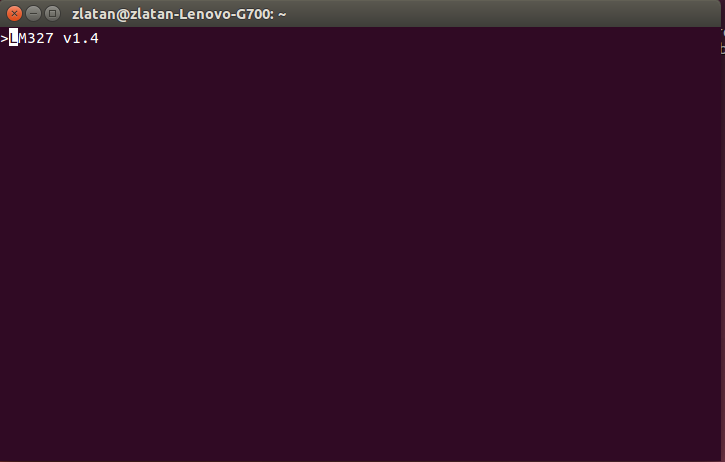
\includegraphics{images/image07.png}}

{As visible on the image above Screen still has issues with carriage
returns.}

{Naturally the next step was to try requesting trouble codes which was
also successfully accomplished. An ignition coil failure simulation was
caused by simply removing the power of one of the ignition coils of the
tested vehicle. The requested temporary DTCs mirrored the anticipated
ignition coil failure code as hexadecimal value. ~}

{}

{\ldots{}\ldots{}\ldots{}\ldots{}\ldots{}\ldots{}\ldots{}\ldots{}\ldots{}\ldots{}\ldots{}\ldots{}..insert
picture here
\ldots{}\ldots{}\ldots{}\ldots{}\ldots{}\ldots{}\ldots{}\ldots{}\ldots{}\ldots{}\ldots{}\ldots{}\ldots{}..}\textsuperscript{\protect\hyperlink{cmnt12}{{[}l{]}}}

{}

{The different }{open source libraries, like
libusb}\textsuperscript{\protect\hyperlink{ftnt5}{{[}5{]}}}{, brought
the capability of getting all devices and their information like vendor
and product ID. Furthermore a simple algorithm searching the sysfs of
Linux provided the associated terminal file path (/dev/tty\ldots{}).
Last but not least the operations of reading and writing were achieved
by the simple file descriptor system calls }{read}{~and }{write}{~in
combination with
}{termios}\textsuperscript{\protect\hyperlink{ftnt6}{{[}6{]}}}{~for
setting the baud rate of these operations. USB normally does not offer
the ability of defining baud rates. This issue originated from the need
of FTDI devices for RS232 ports. Therefore most external hardware, like
Arduino, based on such chips, integrate a RS232 to USB converter
requesting a communication baud rate. Additional research revealed the
}{libftdi}{~library, used exactly for these serial communication issues
with USB. It combines functionalities of libusb with serial
configurations like setting the baud rate. }

{The usage of }{libftdi }{was momentarily discarded, due to no apparent
benefit and the ~additional disadvantage of refactoring the already
existing code. The needed functionality was already covered by combining
the }{libusb }{package with TTY Linux driver and file descriptors.}

\hypertarget{h.nfl0zlavkqps}{\subsubsection{\texorpdfstring{{Emulation}}{Emulation}}\label{h.nfl0zlavkqps}}

{The first approach consisted of exploiting the USBIP API, which
provides the functionality of sharing USB devices over a network. After
assessing its feasibility the decision was made to use the base library
}{libusb-vhci}\textsuperscript{\protect\hyperlink{ftnt7}{{[}7{]}}}{.}

{The }{VHCI}{~project can be described as a driver.
}{VHCI}{~(Vir}{tu}{al Host Controller Interface) is a kernel module with
the capability of emulating a USB hardware device to the kernel. Kernel
modules are code modules executed in the kernel space. They need to be
compiled on each Linux kernel independently to match its structure.
Furthermore the functionalities defined by kernel modules have to be
executed with root privileges.}

{Although compiling the kernel module on each Linux distribution
individually and executing the emulation as root can be rated as a
disadvantage, it is capable of freely emulating USB devices and using
the full scope of USB features defined in the USB
standard}\textsuperscript{\protect\hyperlink{ftnt8}{{[}8{]}}}{. }

{The already existing example code of the project emulates a simple
}{HID }{(Human Interface Device) which mostly covered the needs of the
project. Nevertheless, gradually refactoring the example code led to an
emulation of an }{FTDI}{~device. The result is comprised of three
classes representing the emulation:}

\begin{itemize}
\tightlist
\item
  {USBEmulationSupervisor}
\item
  {USBRequestHandler}
\item
  {EmulatedDevice}
\end{itemize}

{The supervisor handles the general setup of the }{VHCI}{~structure,
including work requests and distribution of different USB
functionalities as well as the request handler. The request handler's
responsibility lies with parsing the USB requests and storing them in an
instance of ``EmulatedDevice'' and responding accordingly to the
request. Currently only one emulated device is possible at a time. The
emulated device holds the device-, configuration- and language
descriptors as well as the function pointer defining the callback. This
callback is meant for giving free possibility of defining what shall
happen on a specific command. Especially ELM commands are of interest
since OBD commands are standardised. The implementation covers only the
most essential functionalities of the }{VHCI}{~library}{.}

{The inconvenience of needing administrator rights discourages the
utilization of the emulation. This issue is unavoidable, since libusb
and libusb\_vhci both use functionalities, like claiming a hardware
device, which require administrator rights. The fully functional
software is intended to have its suid bit set once, therefore granting
it administrator rights by default or at least ensuring that it has to
be executed as administrator.}

{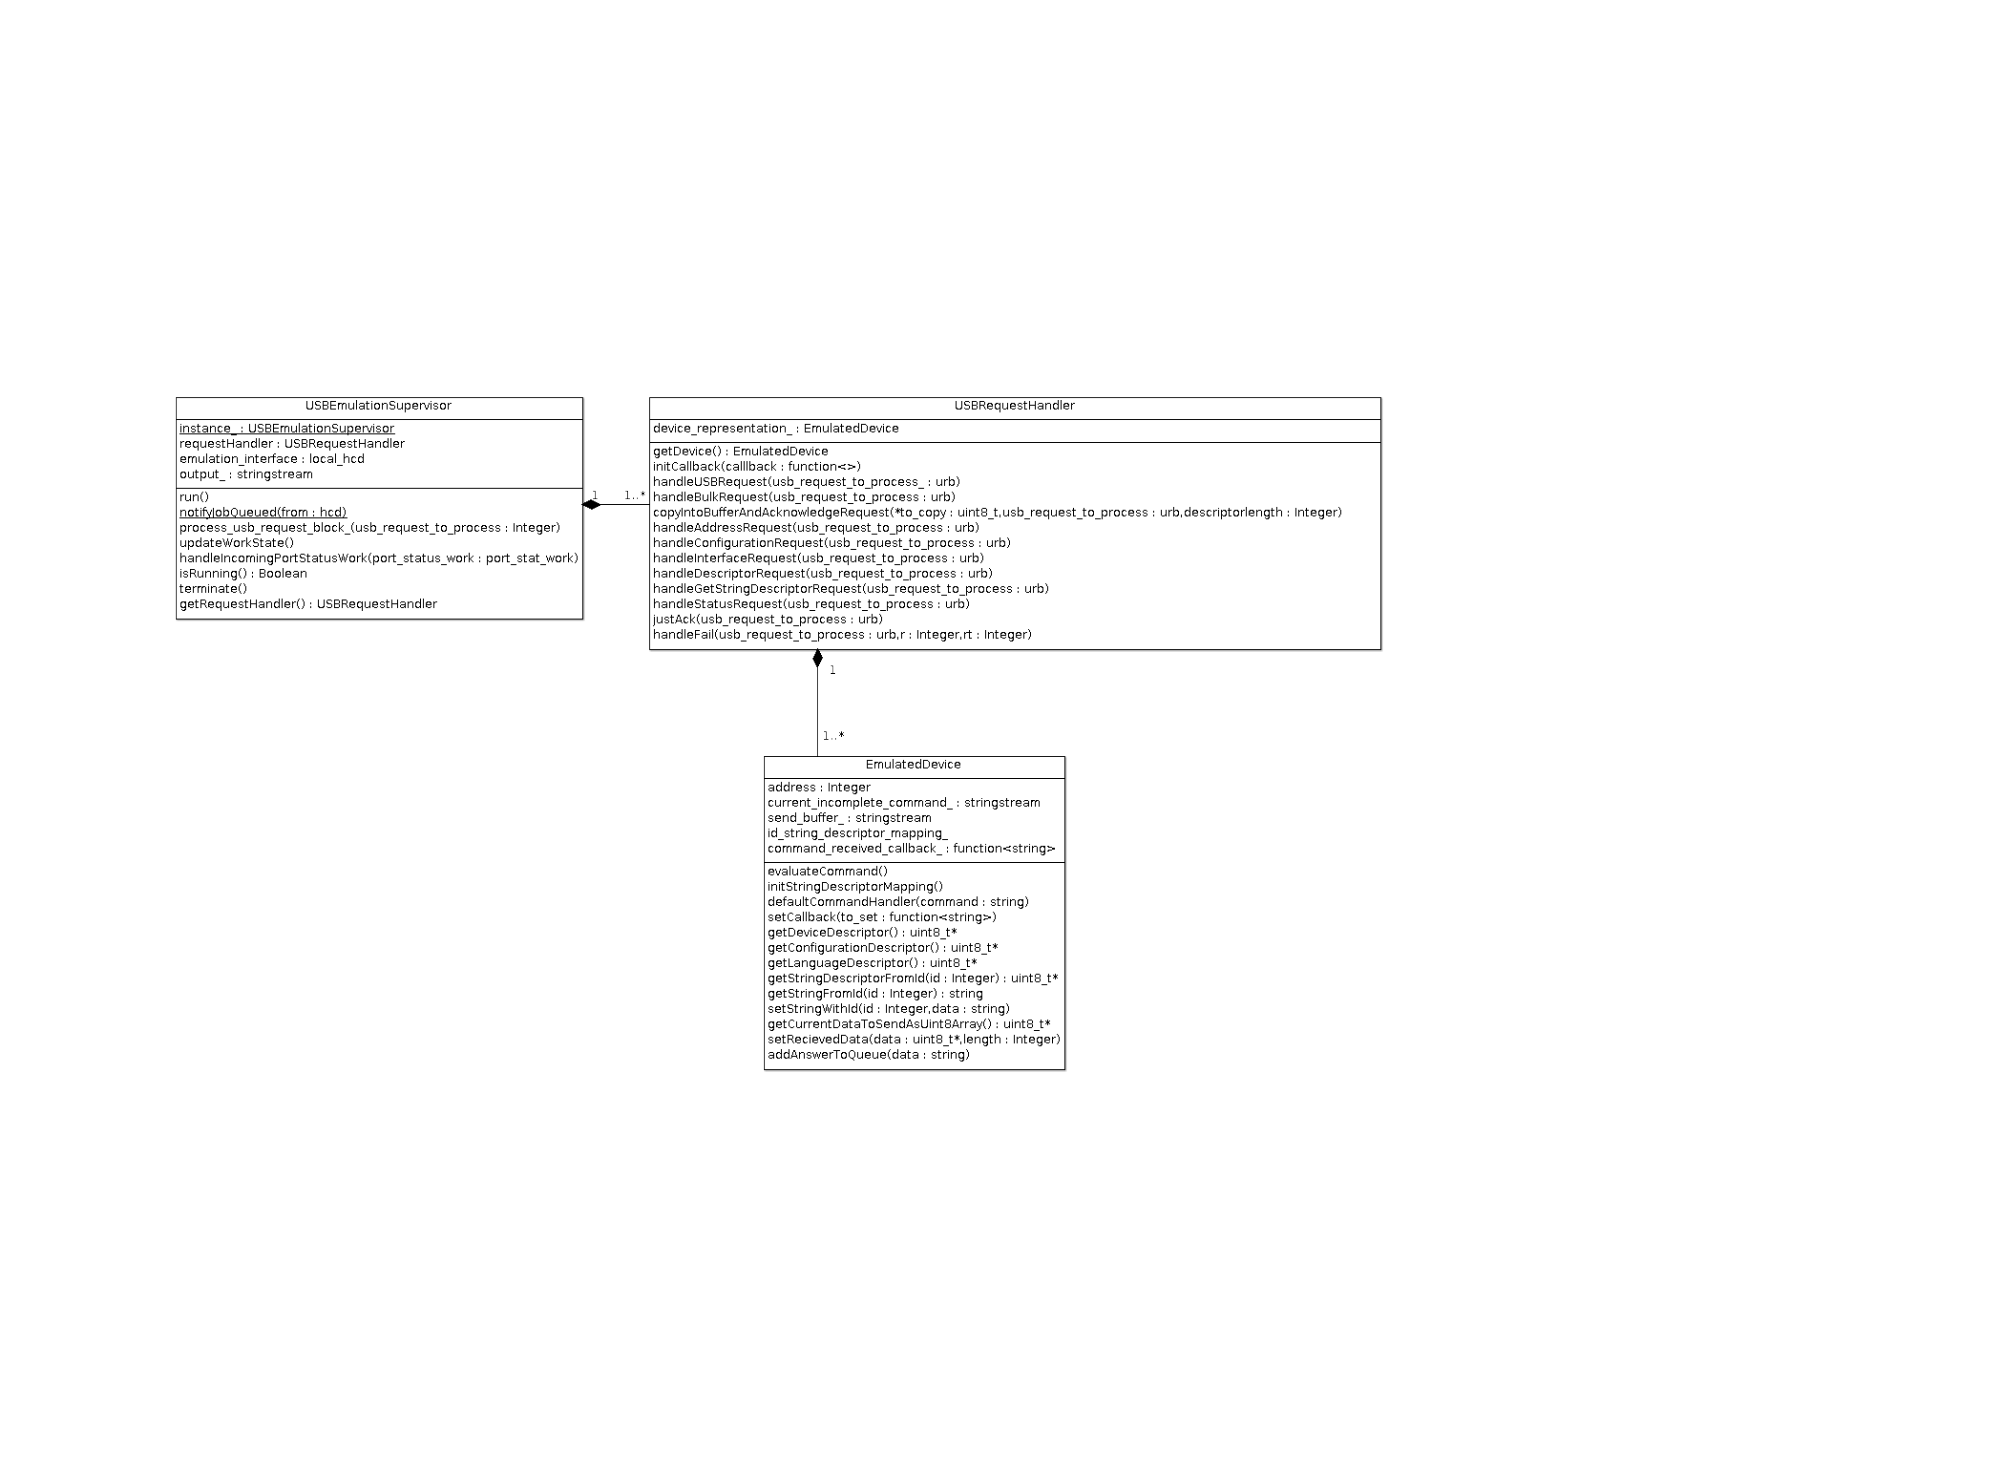
\includegraphics{images/image04.png}}

\hypertarget{h.rpls244qrcic}{\subsection{\texorpdfstring{{Databases}\textsuperscript{\protect\hyperlink{cmnt13}{{[}m{]}}}}{Databases{[}m{]}}}\label{h.rpls244qrcic}}

{Storing and managing data is bound to become an issue due to the
enormous amount of data sets in in relation to OBD. Therefore a
thoroughly implemented database interface cannot be avoided. For reasons
of simplicity the base query language for the database MySQL was chosen.
The main advantages leading to the choice of MySQL is the easy
installation of MySQL server and client on all Linux distributions as
well as the API availability.
MySQLConnector++}\textsuperscript{\protect\hyperlink{ftnt9}{{[}9{]}}}{~is
a C++ API for MySQL, which supplies the basic framework for executing
and parsing responses of any database. Since it is an external library
~}{\protect\hyperlink{h.v0k64l3n1ort}{Clean Code}}{~advises }{to wrap
its API in a self defined interface, which is represented by this
subpackage. }

{The general structure composes of a class responsible for dispatching
the requests, a class for parsing the data into a C++ conform class
structure as well as an executor class defining the insertion and
deletion commands. Keeping the philosophy of TDD (Test Driven
Development) in mind it seemed wise to setup a test database as an SQL
dump and supply a script reinitiating the database. After a testing
function has manipulated the database this script can be used to reset
the test database to its initial state. }

{The configuration parameters can either be entered hardcoded or by
parsing an XML file containing the host address, user, password and
database name. The parsing ~structure is thoroughly explained in the
}{\protect\hyperlink{h.ndb5fg1te708}{Configuration}}{~section. The XML
looks as follows:}

{}

{\textless{}?}{xml
version}{=}{``1.0''}{~encoding}{=}{``UTF-8''}{?\textgreater{}}

{\textless{}!DOCTYPE database SYSTEM ``database.dtd''\textgreater{}}

{\textless{}database\textgreater{}}

{~~~~~~~~}{\textless{}address\textgreater{}}{127.0.0.1}{\textless{}/address\textgreater{}}

{~~~~~~~~}{\textless{}user\textgreater{}}{obd}{\textless{}/user\textgreater{}}

{~~~~~~~~}{\textless{}password\textgreater{}\textless{}/password\textgreater{}}

{~~~~~~~~}{\textless{}dbname\textgreater{}}{OBD\_TroubleCodes}{\textless{}/dbname\textgreater{}}

{\textless{}/database\textgreater{}}

{The password field is left empty as the user obd has no password setup.
~}

{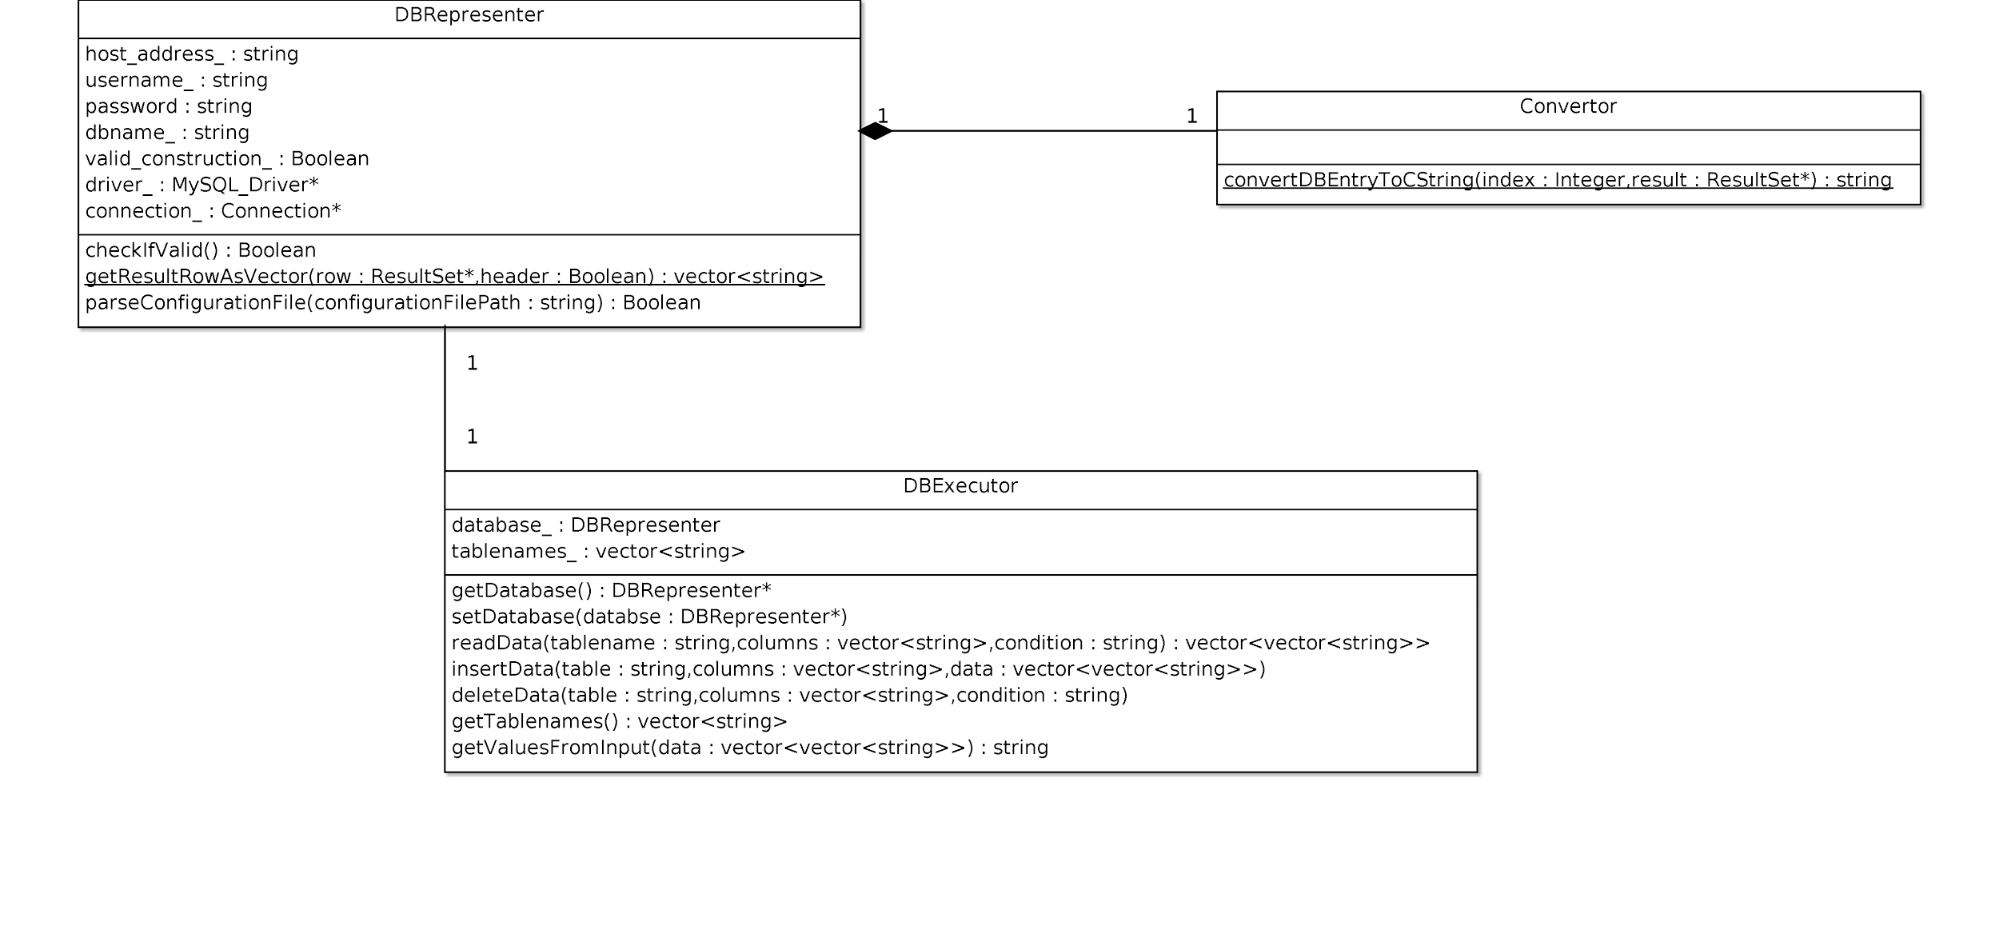
\includegraphics{images/image10.png}}

\hypertarget{h.fbh3ldin73fx}{\subsection{\texorpdfstring{{OBD
Base}\textsuperscript{\protect\hyperlink{cmnt14}{{[}n{]}}}}{OBD Base{[}n{]}}}\label{h.fbh3ldin73fx}}

{The OBDBase package represents the OBD specific part of this thesis. It
provides links between the OBD structures like hexadecimal responses
from the ELM to the database entries with their column definitions and
IDs, as well as calculations, minimum and maximum values of single
sensors and ELM specific command representations.}

{The OBD interface responds to PIDs of service mode I and II with a
certain amount of bytes. This amount is defined in the ISO 15031
depending on the sensor the PID represents. PIDs that are modulo 32 are
requests to get a 32 bit value of implemented PIDs of the next 32 PIDs.
Meaning PID 0 (e.g. 01 00) returns four bytes where each bit is
interpreted as a boolean value, stating the availability of the
corresponding PID. The interpretation of these received bytes is defined
in the above mentioned ISO standard as well. Analyzing the accessible
PIDs a grouping into four different value types could be extracted.}

\hypertarget{h.tbf8n411o12j}{\subsubsection{\texorpdfstring{{Calculation
Values}}{Calculation Values}}\label{h.tbf8n411o12j}}

{Calculation values are responses or part of a response, where the
received value represents the value of the specific PID's underlying
entity. As the name suggests there are additional calculations
necessary. The standard defines the environment parameters of these
values, which are supplied by an XML file. PID 0x66 shows an example of
a calculation value:}

{\textless{}value}{~}{interpretation}{=}{``calculation''\textgreater{}}

{~ }{\textless{}name\textgreater{}}{MAF Sensor
A}{\textless{}/name\textgreater{}}

{~ \textless{}bytes\textgreater{}}{2}{\textless{}/bytes\textgreater{}}

{~~~~~~~~~
}{\textless{}min\textgreater{}}{0}{\textless{}/min\textgreater{}}

{~
\textless{}max\textgreater{}}{2047.96875}{\textless{}/max\textgreater{}}

{~ \textless{}unit\textgreater{}}{g/s}{\textless{}/unit\textgreater{}}

{\textless{}/value\textgreater{}}

{These definitions describe the range of the received data, in this case
from 0 - 2047.96875 g/s for 0 - 65535 decimal value of two bytes. This
means that a received byte value of 0 corresponds to 0 g/s and a decimal
value of 65535 represents 2047.9687 g/s. When resolving these relations
the following formula can be used for converting values: }

{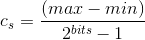
\includegraphics{images/image08.png}}

{~}{
\includegraphics{images/image00.png}}

{}

{void}{~}{OBDCalculationValue}{::}{interpretCalculationValue}{(}{std}{::}{vector}{\textless{}uint8\_t\textgreater{}}{~input)}

{\{}

{~ ~ }{unsigned}{~}{int}{~compound\_value
}{=}{~calculateCompoundValue}{(}{input}{);}

{~ ~ }{double}{~scale }{=}{~}{(}{max\_
}{-}{~min\_}{)}{~}{/}{~}{(}{pow}{(}{2.0}{,}{~byte\_amount\_
}{*}{~}{8.0}{)}{~}{-}{~}{1}{);}

{~ ~ interpreted\_value\_ }{=}{~compound\_value }{*}{~scale
}{+}{~min\_;}

{~ ~ uninterpreted\_value\_ }{=}{~compound\_value;}

{\}}

{The conversion of interpreted values to raw values ~naturally deduces:}

\begin{center}\rule{0.5\linewidth}{\linethickness}\end{center}

{}

{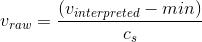
\includegraphics{images/image01.png}}

{void}{~}{OBDCalculationValue}{::}{interpretCalculationByteArray}{(}{double}{~value)}

{\{}

{~ ~ interpreted\_value\_ }{=}{~value;}

{~ ~ interpreted\_value\_
}{=}{~std}{::}{min}{(}{interpreted\_value\_}{,}{~max\_}{);}

{~ ~ interpreted\_value\_
}{=}{~std}{::}{max}{(}{interpreted\_value\_}{,}{~min\_}{);}

{~ ~ }{double}{~scale }{=}{~}{(}{max\_
}{-}{~min\_}{)}{~}{/}{~}{(}{pow}{(}{2.0}{,}{~byte\_amount\_
}{*}{~}{8.0}{)}{~}{-}{~}{1}{);}

{~ ~ uninterpreted\_value\_ }{=}{~}{(}{interpreted\_value\_
}{-}{~min\_}{)}{~}{/}{~scale;}

{\}}

\hypertarget{h.t1w3v8o28dma}{\subsubsection{\texorpdfstring{{Value
Mapping Values}}{Value Mapping Values}}\label{h.t1w3v8o28dma}}

{These are values whose raw values are used on a predefined mapping to
get a string representation of this specific PID's request. Meaning the
value directly maps to a result string. The configuration of such a
value requires only the mapping itself, as illustrated by the PID 0x5f:}

{\textless{}value}{~}{interpretation}{=}{``mapping''\textgreater{}}

{~ }{\textless{}bytes\textgreater{}}{1}{\textless{}/bytes\textgreater{}}

{~~~~~~~~~ }{\textless{}mapping}{~}{type}{=}{``value''\textgreater{}}

{~ ~ }{\textless{}entry}{~}{from}{=}{``0E''}{\textgreater{}}{LKW (Euro
IV) B1}{\textless{}/entry\textgreater{}}

{~~~~~~~~~ ~ }{\textless{}entry}{~}{from}{=}{``0F''}{\textgreater{}}{LKW
(Euro V) B2}{\textless{}/entry\textgreater{}}

{~~~~~~~~~ ~ }{\textless{}entry}{~}{from}{=}{``10''}{\textgreater{}}{LKW
(Euro EEV) C}{\textless{}/entry\textgreater{}}

{~ ~}{\textless{}/mapping\textgreater{}}{~~~~~~~~~~~~~~~~}

{\textless{}/value\textgreater{}}

\hypertarget{h.nvvniy6ibvmm}{\subsubsection{\texorpdfstring{{Bit Mapping
Values}}{Bit Mapping Values}}\label{h.nvvniy6ibvmm}}

{As the name suggests bit mapping values are values, where each bit has
a different meaning. Information required from the ISO standard is only
the mapping and significance of the single bits. In some cases a bits
true and false value signify different outputs for the same entity. An
example of such a value is PID 0 as well as PID 0x65.}

\begin{center}\rule{0.5\linewidth}{\linethickness}\end{center}

{}

{\textless{}value}{~}{interpretation}{=}{``mapping''\textgreater{}}

{~ }{\textless{}bytes\textgreater{}}{1}{\textless{}/bytes\textgreater{}}

{~ }{\textless{}mapping}{~}{type}{=}{``bit''\textgreater{}}

{~ ~
}{\textless{}entry}{~}{from}{=}{``0''}{~}{set}{=}{``false''}{\textgreater{}}{Kraftaufnahme
inaktiv}{\textless{}/entry\textgreater{}}

{~ ~
}{\textless{}entry}{~}{from}{=}{``0''}{~}{set}{=}{``true''}{\textgreater{}}{Kraftaufnahme
aktiv}{\textless{}/entry\textgreater{}}

{~ ~
}{\textless{}entry}{~}{from}{=}{``1''}{~}{set}{=}{``false''}{\textgreater{}}{Automatikgetriebe
in Park-/Neutralstellung}{\textless{}/entry\textgreater{}}

{~ ~
}{\textless{}entry}{~}{from}{=}{``1''}{~}{set}{=}{``true''}{\textgreater{}}{Vorwärts-
oder Rückwärtsgang}{\textless{}/entry\textgreater{}}

{~ ~
}{\textless{}entry}{~}{from}{=}{``2''}{~}{set}{=}{``false''}{\textgreater{}}{Manuelles
Getriebe in \ldots{} Kupplung getreten}{\textless{}/entry\textgreater{}}

{~ ~
}{\textless{}entry}{~}{from}{=}{``2''}{~}{set}{=}{``true''}{\textgreater{}}{Gang
eingelegt}{\textless{}/entry\textgreater{}}

{~ ~
}{\textless{}entry}{~}{from}{=}{``3''}{~}{set}{=}{``false''}{\textgreater{}}{Vorglühlampe
aus}{\textless{}/entry\textgreater{}}

{~ ~
}{\textless{}entry}{~}{from}{=}{``3''}{~}{set}{=}{``true''}{\textgreater{}}{Lampe
ein}{\textless{}/entry\textgreater{}}

{~ }{\textless{}/mapping\textgreater{}}

{\textless{}/value\textgreater{}}

{The from field specifies the bit position while the set attribute is an
optional attribute to assign a bits value to a concrete output. In this
case it is supplied, meaning that depending ~on the bits status
different strings are mapped. If the set attribute is not explicitly
stated it is assumed true.}

{std}{::}{string}{~}{OBDBitMappingValue}{::}{interpretToValue}{(}{std}{::}{vector}{\textless{}uint8\_t\textgreater{}}{~input)}

{\{}

{~ ~ interpreted\_value\_ }{=}{~calculateCompoundValue}{(}{input}{);}

{~ ~ uninterpreted\_value\_ }{=}{~interpreted\_value\_;}

{~ ~ }{return}{~getInterpretedValueAsString}{();}

{\}}

{As}{~this code shows in case of mapping values of interpreted and
uninterpreted values are identic}{al and represent the key of the
underlying mapping.}

\hypertarget{h.v3wlh8gjmo1s}{\subsubsection{\texorpdfstring{{Bit
Combination Mapping
Values}}{Bit Combination Mapping Values}}\label{h.v3wlh8gjmo1s}}

{This value parsing is a bit comparator mapping of more than two bits.
The from field specifies the bit positions and the set represents the
value it needs to equal to get the result string in question. PID 0x70
is an example of such a mapping.}

{\textless{}value}{~}{interpretation}{=}{``mapping''\textgreater{}}

{~ ~
}{\textless{}bytes\textgreater{}}{1}{\textless{}/bytes\textgreater{}}

{~ ~ }{\textless{}mapping}{~}{type}{=}{``bitcombination''\textgreater{}}

{~ ~ ~ ~
}{\textless{}validitybit}{~}{from}{=}{``01''}{\textgreater{}}{2}{\textless{}/validitybit\textgreater{}}

{~ ~ ~ ~
}{\textless{}entry}{~}{from}{=}{``01''}{~}{set}{=}{``01''}{\textgreater{}}{Offener
Kreislauf, kein Fehler}{\textless{}/entry\textgreater{}}

{~ ~ ~ ~
}{\textless{}entry}{~}{from}{=}{``01''}{~}{set}{=}{``10''}{\textgreater{}}{Geschlossener
Kreislauf, kein Fehler}{\textless{}/entry\textgreater{}}

{~ ~ ~ ~
}{\textless{}entry}{~}{from}{=}{``01''}{~}{set}{=}{``11''}{\textgreater{}}{Fehler
vorhanden, Wert unzuverlässig}{\textless{}/entry\textgreater{}}

{~ ~ ~ ~
}{\textless{}validitybit}{~}{from}{=}{``23''}{\textgreater{}}{5}{\textless{}/validitybit\textgreater{}}

{~ ~ ~ ~
}{\textless{}entry}{~}{from}{=}{``23''}{~}{set}{=}{``01''}{\textgreater{}}{Offener
Kreislauf, kein Fehler}{\textless{}/entry\textgreater{}}

{~ ~ ~ ~
}{\textless{}entry}{~}{from}{=}{``23''}{~}{set}{=}{``10''}{\textgreater{}}{Geschlossener
Kreislauf, kein Fehler}{\textless{}/entry\textgreater{}}

{~ ~ ~ ~
}{\textless{}entry}{~}{from}{=}{``23''}{~}{set}{=}{``11''}{\textgreater{}}{Fehler
vorhanden, Wert unzuverlässig}{\textless{}/entry\textgreater{}}

{~ ~ }{\textless{}/mapping\textgreater{}}{~ ~ }

{\textless{}/value\textgreater{}}

\hypertarget{h.q2wfq2ktke27}{\subsubsection{\texorpdfstring{{Inner
Workings}}{Inner Workings}}\label{h.q2wfq2ktke27}}

{Since most PIDs do not consist of only one value or type, values have
to be defined in the order they are supposed to be received. They can be
combined as needed, so that multiple calculation values can be followed
by any mapping value or vice versa. The total of the single value
definition's bytes will then be expected when parsing the OBD commands
answer, giving significance to the order of the sequence in which the
values are defined in the XML file.}

{\textless{}obdcommand\textgreater{}}

{~ }{\textless{}pid\textgreater{}}{70}{\textless{}/pid\textgreater{}}

{~
}{\textless{}description\textgreater{}}{Ladedruckregelung}{\textless{}/description\textgreater{}}

{~ }{\textless{}validitymapping}{~
}{mode}{=}{``manual''}{\textgreater{}}{true}{\textless{}/validitymapping\textgreater{}}

{~ }{\textless{}values\textgreater{}}

{~ ~
}{\textless{}value}{~}{interpretation}{=}{``calculation''\textgreater{}}

{~ ~ ~ }{\textless{}name\textgreater{}}{Soll Ladedruck
A}{\textless{}/name\textgreater{}}

{~ ~ ~
}{\textless{}bytes\textgreater{}}{2}{\textless{}/bytes\textgreater{}}

{~ ~ ~ }{\textless{}min\textgreater{}}{0}{\textless{}/min\textgreater{}}

{~ ~ ~
}{\textless{}max\textgreater{}}{2047.96875}{\textless{}/max\textgreater{}}

{~ ~ ~
}{\textless{}unit\textgreater{}}{kPa}{\textless{}/unit\textgreater{}}

{~ ~ ~
}{\textless{}validitybit\textgreater{}}{0}{\textless{}/validitybit\textgreater{}~~~~~~~~}

{~ ~ }{\textless{}/value\textgreater{}}

{~ ~
}{\textless{}value}{~}{interpretation}{=}{``calculation''\textgreater{}}

{~ ~ ~ }{\textless{}name\textgreater{}}{Ist Ladedruck
A}{\textless{}/name\textgreater{}}

{~ ~ ~
}{\textless{}bytes\textgreater{}}{2}{\textless{}/bytes\textgreater{}}

{~ ~ ~ }{\textless{}min\textgreater{}}{0}{\textless{}/min\textgreater{}}

{~ ~ ~
}{\textless{}max\textgreater{}}{2047.96875}{\textless{}/max\textgreater{}}

{~ ~ ~
}{\textless{}unit\textgreater{}}{kPa}{\textless{}/unit\textgreater{}~~~~~~~~}

{~ ~ ~
}{\textless{}validitybit\textgreater{}}{1}{\textless{}/validitybit\textgreater{}}{~~~~~~~~~~~~~~~~~~~~~~~~}

{~ ~ }{\textless{}/value\textgreater{}}

{~ ~ }{.}

{~ ~ }{.}

{~ ~ }{.}

{~ ~
}{\textless{}value}{~}{interpretation}{=}{``mapping''\textgreater{}}

{~ ~ ~
}{\textless{}bytes\textgreater{}}{1}{\textless{}/bytes\textgreater{}}

{~ ~ ~
}{\textless{}mapping}{~}{type}{=}{``bitcombination''\textgreater{}}

{~ ~ ~ ~
}{\textless{}validitybit}{~}{from}{=}{``01''}{\textgreater{}}{2}{\textless{}/validitybit\textgreater{}}

{~ ~ ~ ~
}{\textless{}entry}{~}{from}{=}{``01''}{~}{set}{=}{``01''}{\textgreater{}}{Offener
Kreislauf, kein Fehler}{\textless{}/entry\textgreater{}}

{~ ~ ~ ~
}{\textless{}entry}{~}{from}{=}{``01''}{~}{set}{=}{``10''}{\textgreater{}}{Geschlossener
Kreislauf, kein Fehler}{\textless{}/entry\textgreater{}}

{~ ~ ~ ~
}{\textless{}entry}{~}{from}{=}{``01''}{~}{set}{=}{``11''}{\textgreater{}}{Fehler
vorhanden, Wert unzuverlässig}{\textless{}/entry\textgreater{}}

{~ ~ ~ ~
}{\textless{}validitybit}{~}{from}{=}{``23''}{\textgreater{}}{5}{\textless{}/validitybit\textgreater{}}

{~ ~ ~ ~
}{\textless{}entry}{~}{from}{=}{``23''}{~}{set}{=}{``01''}{\textgreater{}}{Offener
Kreislauf, kein Fehler}{\textless{}/entry\textgreater{}}

{~ ~ ~ ~
}{\textless{}entry}{~}{from}{=}{``23''}{~}{set}{=}{``10''}{\textgreater{}}{Geschlossener
Kreislauf, kein Fehler}{\textless{}/entry\textgreater{}}

{~ ~ ~ ~
}{\textless{}entry}{~}{from}{=}{``23''}{~}{set}{=}{``11''}{\textgreater{}}{Fehler
vorhanden, Wert unzuverlässig}{\textless{}/entry\textgreater{}}

{~ ~ ~ }{\textless{}/mapping\textgreater{}}{~~~~~~~~~~~~~~~~}

{~ ~ }{\textless{}/value\textgreater{}}

{~ }{\textless{}/values\textgreater{}}

{\textless{}/obdcommand\textgreater{}}

{Furthermore special OBD commands exist where the first byte defines
which of the transmitted following bytes are valid values. These OBD
commands are mostly used for array sensor PIDs. The package offers
therefore the optional definition of an automatic or manual validity
mapping. }

{A validity mapping contains one or more bytes beginning the response in
which the position of the bits correspond to the following bytes and
their value. The value on a certain position in this mapping byte
indicates if the transmitted value is valid or can be ignored.}

{There are no rules without exceptions. Certain values have a complex
validity mapping structure especially in association with the bit
combination mapping. Therefore the need for manually configurable
validity mapping emerged which got implemented as the manual validity
mapping mode. The amount of such values is limited (one or two
occurrences). In this mode the validity bit position has to be defined
separately with a tag in the all corresponding value definition. }

{High abstraction is achieved with an abstract base class. It defines
main utility functions like adding bytes to a compound value, storing
the raw and interpreted data and delegating the interpretation trough a
pure virtual function to its derived classes. }

{A simple factory pattern which creates OBDCommandValues from its XML
representation ensures easy usability. It creates the values depending
on the interpretation attribute of each value tags definition and
returns an abstract object representing the value. }

\hypertarget{h.wbiklph9gdnl}{\subsubsection{\texorpdfstring{{ELM
Commands}}{ELM Commands}}\label{h.wbiklph9gdnl}}

{There is a set of ELM specific commands configurable for the
communication to the control unit of the automobile. Generally the
emulation has to answer those requests and the OBD tool must configure
the ELM specific settings. Therefore it seemed necessary to implement a
parsing and object representation of the ElmCommands for our middleware
package.}

{The difficulty of this part of the OBDBase package surfaced when
inspecting the single commands more closely. The datasheet of the ELM
offered an inconsistent way of defining additional values. In most cases
they are referenced as ``h'' (hexadecimal value) but there are some
values referenced by ``x'','' y'' or ``z'' as well.}

{\textless{}command\textgreater{}}

{~
}{\textless{}version\textgreater{}}{1.0}{\textless{}/version\textgreater{}}

{~
}{\textless{}elmcommand\textgreater{}}{``AL''}{\textless{}/elmcommand\textgreater{}}

{~ }{\textless{}description\textgreater{}}{``Allow Long (\textgreater{}7
byte) messages''}{\textless{}/description\textgreater{} }

{~
}{\textless{}group\textgreater{}}{``OBD''}{\textless{}/group\textgreater{}}

{\textless{}/command\textgreater{}}

\hypertarget{h.8c6emwe3lhuv}{\subsection{\texorpdfstring{{Configuration}}{Configuration}}\label{h.8c6emwe3lhuv}}

{The configuration subpackage is used to parse and write XML files.
Currently there are following configuration files: }

\begin{itemize}
\tightlist
\item
  {elmcommandconfiguration.xml}
\item
  {obdcommand.xml}
\item
  {obdcuConfiguration.xml}
\item
  {obdtoolConfiguration.xml}
\item
  {dbconfiguration.xml}
\end{itemize}

{These contain configuration parameters for the software. The command
configurations (elmcommandconfiguration.xml and odbcommand.xml) contain
all commands known by the ELM327 extracted from its
datasheet}\textsuperscript{\protect\hyperlink{ftnt10}{{[}10{]}}}{~or all
OBD commands consisting of service ID with its corresponding PID and
name. The project configurations (obdcuConfiguration.xml and
obdtoolConfiguration.xml) are only path declarations to the other
configurations enabling factory resets.}

{This package uses the functionalities of the libxml++
library}\textsuperscript{\protect\hyperlink{ftnt11}{{[}11{]}}}{. This
library uses the DOM (Document Object Model) and supplies
functionalities for parsing an XML file into a DOM model as well as
writing a DOM model to a file. }

{The base of the configuration package consists of the XMLWriter,
XMLReader and DefaultHandler classes. Their purpose is to parse a DOM
object into internal class representations, as suggested in
}{\protect\hyperlink{h.mifm7q3zf07v}{Clean Code}}{, therefore
simplifying the usage of the libxml++ library functions to creating a
derived class of the DefaultXMLHandler. }

{This class has a pure virtual method handleNode which gets a
xmlpp::Node* as parameter. A derived class instance can distinguish its
execution and parsing behavior by comparing e.g. the name of the
xmlpp::Node. The DefaultXMLHandler supplies protected functions for
parsing xmlpp::TextNode* into C++ strings or
}{setting}{~xmlpp::TextNode* from C++ strings. }

{Handlers only define the handling of the nodes, more precisely setting
~or parsing the underlying libxml++ DOM representation
(xmlpp::Document). The XMLWriter and XMLReader classes are initialized
with an instance of the DefaultXMLHandler. Its parse or write function
requires an already existing XML file. Each function calls its
internally defined DefaultHandler's handleNode function while
recursively iterating through DOM nodes. A well formed ~structure of the
underlying XML files is ensured by the required DTD files, shown
beneath, ~defining the structure of the XML files.}

{}

\href{}{}\href{}{}

\begin{longtable}[]{@{}ll@{}}
\toprule
\begin{minipage}[t]{0.47\columnwidth}\raggedright\strut
{XML}
\strut\end{minipage} &
\begin{minipage}[t]{0.47\columnwidth}\raggedright\strut
{DTD}
\strut\end{minipage}\tabularnewline
\begin{minipage}[t]{0.47\columnwidth}\raggedright\strut
{\textless{}?}{xml
version}{=}{``1.0''}{~encoding}{=}{``UTF-8''}{?\textgreater{}}

{\textless{}!DOCTYPE database SYSTEM ``database.dtd''\textgreater{}}

{}

{\textless{}database\textgreater{}}

{~~~~~~~~}{\textless{}address\textgreater{}}{127.0.0.1}{\textless{}/address\textgreater{}}

{~~~~~~~~}{\textless{}user\textgreater{}}{obd}{\textless{}/user\textgreater{}}

{~~~~~~~~}{\textless{}password\textgreater{}\textless{}/password\textgreater{}}

{~~~~~~~~}{\textless{}dbname\textgreater{}}{OBD\_TroubleCodes}{\textless{}/dbname\textgreater{}}

{\textless{}/database\textgreater{}}
\strut\end{minipage} &
\begin{minipage}[t]{0.47\columnwidth}\raggedright\strut
{\textless{}!ELEMENT database (address, user, password,
dbname)\textgreater{}}

{\textless{}!ELEMENT address (\#PCDATA)\textgreater{}}

{\textless{}!ELEMENT user (\#PCDATA)\textgreater{}}

{\textless{}!ELEMENT password (\#PCDATA)\textgreater{}}

{\textless{}!ELEMENT dbname (\#PCDATA)\textgreater{}}
\strut\end{minipage}\tabularnewline
\bottomrule
\end{longtable}

{The difference between the two classes is that, whilst the XMLReader
only iterates and lets the handler save the read data, the XMLWriter
sets the DefaultHandler into a mode, where he instead of parsing the
node's data sets it. After the iteration the XMLWriter writes to the
same file it read from with the newly filled data. }

{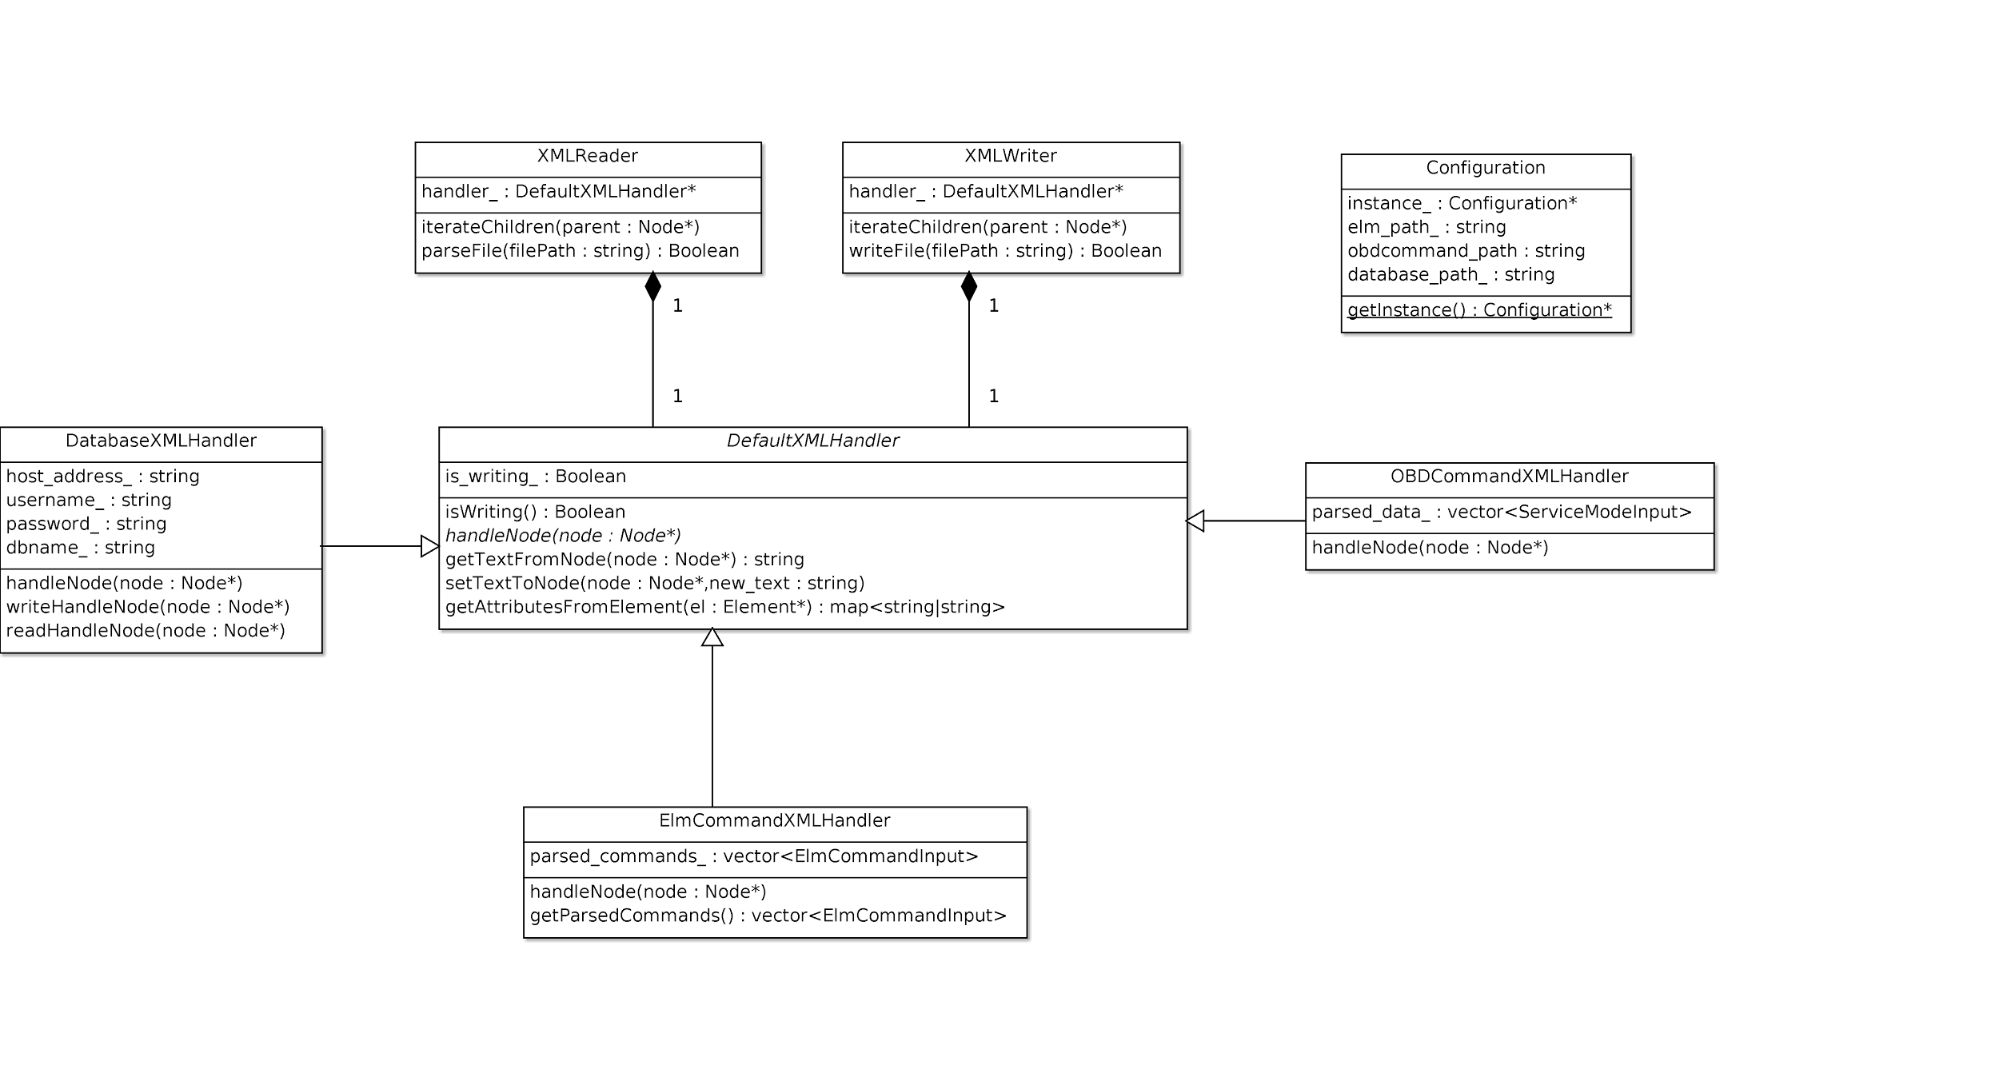
\includegraphics{images/image03.png}}

{}

\hypertarget{h.upb9og5wn4q0}{\section{\texorpdfstring{{Project Specific
Implementation}\textsuperscript{\protect\hyperlink{cmnt15}{{[}o{]}}}}{Project Specific Implementation{[}o{]}}}\label{h.upb9og5wn4q0}}

{The preceding package implementation descriptions only focus on
overlapping functionalities. The result is the OBDMiddleware package
which is an API. Furthermore a concrete application has to be
implemented to apply the designed features. The OBDCU, which stands for
On Board Diagnosis Control Unit, represents the emulated diagnosis CU.
It offers possibilities to emulate attached USB devices on Linux systems
and is able to set and unset permanent and pending diagnostic trouble
codes as well as deleting them. The OBD tool was supposed to be its
counterpart for reading trouble codes and its corresponding freeze frame
data, but since our time contingent did not suffice the OBD tool as well
as the OBDCU's sensor capabilities were not implemented. Although it is
safe to say that the general functionalities for requesting sensor data
is included in the OBDMiddleware. Even though the common mechanics are
asserted by unit tests, the additional implementation and connection of
the related sensor functions would easily overstep the efforts of this
bachelor thesis.}

{CMake ensures easy compilation and first and foremost dependencies to
external packages in combination with the usage of self implemented
packages. A setup for development was provided by making paths to the
subprojects configurable. Packaging for installation was ensured by
using CPack generators, especially for Debian systems. }

{The Model-View-Controller architecture was chosen due to its clear
specification of classes and their clustering into general divisions.
The model being the middleware package itself.}

\hypertarget{h.dfu1gktb8xw}{\subsection{\texorpdfstring{{OBDCU}\textsuperscript{\protect\hyperlink{cmnt16}{{[}p{]}}}}{OBDCU{[}p{]}}}\label{h.dfu1gktb8xw}}

{The OBDCU application offers the user the possibility to emulate and
partially configure an USB FTDI device with one configuration and one
set of bulk endpoints. Furthermore diagnostic trouble codes are
selectable from a database and settable to the emulated fault memory
either as a permanent or temporary trouble code. Additionally it
supplies a surface to configure responses to ELM commands (e.g. atz).
While the current version only supplies a beta version with several
restrictions regarding the configurations, since they are only saved
over the runtime of the application. However it is able to simulate at
least three of ten service modes as well as all ELM commands. As
previously mentioned service modes one and two are prepared in the
OBDMiddleware package but since the project has already exceeded the
time requirements for a bachelor thesis it seemed reasonable to omit
those parts. }

\hypertarget{h.pxkpe4k3lbn1}{\section{\texorpdfstring{{Installation}\textsuperscript{\protect\hyperlink{cmnt17}{{[}q{]}}}{~How
To}}{Installation{[}q{]}~How To}}\label{h.pxkpe4k3lbn1}}

{Several steps have to be taken before starting or building the project
on a development environment. This project has a lot of dependencies,
which are listed in the built package, and it requires kernel modules.
This section elaborates on additional dependencies and building
instructions depending on the purpose.}

{This project uses different open source API to realize the desired
functionalities. The following packages are included in the official
Ubuntu repositories and can be downloaded by any package management
system:}

\begin{itemize}
\tightlist
\item
  {libmysqlcppconn-dev }
\item
  {mysql-server}
\item
  {libusb }
\item
  {libusb-dev}
\item
  {libxml++2.6-2 }
\item
  {libxml++2.6-2-dev }
\item
  {qt-sdk}
\item
  {libcppunit-dev }
\item
  {libcppunit-1.13-0 }
\item
  {libboost-all-dev }
\end{itemize}

{The only packages which require manual compilation are the libusb-vhci
library and the vhci\_hcd
package}\textsuperscript{\protect\hyperlink{ftnt12}{{[}12{]}}}{,
resulting in two kernel module files (.ko). Those files either have to
be inserted manually using
}{insmod}\textsuperscript{\protect\hyperlink{ftnt13}{{[}13{]}}}{~or they
have to be installed with the help of make install. When installing and
frequently accessing the kernel modules it is advisable to alter the
modules system file, located under ``/etc/modules'', by adding them at
the end of the file. This will result in the loading of the kernel
modules at startup.}

{To compile the libusb-vhci project the following steps have to be
done:}

\hypertarget{h.agltrea2kef8}{\subsubsection{\texorpdfstring{{vhci\_hcd}}{vhci\_hcd}}\label{h.agltrea2kef8}}

\begin{enumerate}
\tightlist
\item
  {download}\textsuperscript{\protect\hyperlink{ftnt14}{{[}14{]}}}{~or
  use from repository}
\item
  {make}
\item
  {sudo make install}
\end{enumerate}

{Optional - depending on how kernel modules want to be handled:}

\begin{enumerate}
\setcounter{enumi}{3}
\tightlist
\item
  {insmod usb-vhci-hcd.ko}
\item
  {insmod usb-vhci-iocifc.ko}
\end{enumerate}

{or:}

\begin{enumerate}
\setcounter{enumi}{3}
\tightlist
\item
  {sudo gedit /etc/modules \&}
\item
  {add kernel module names (without extension) to file and save}
\end{enumerate}

\hypertarget{h.8woybtsjfs8s}{\subsubsection{\texorpdfstring{{libusb\_vhci
(userspace
tools):}}{libusb\_vhci (userspace tools):}}\label{h.8woybtsjfs8s}}

\begin{enumerate}
\tightlist
\item
  {download}\textsuperscript{\protect\hyperlink{ftnt15}{{[}15{]}}}{~or
  use from repository}
\item
  {./configure}
\item
  {make}
\item
  {sudo make install}
\item
  {sudo ldconfig -v }
\end{enumerate}

{Depending on the Linux kernel version}{~}{and the current vhci\_hcd and
libusb\_vhci versions, the compiling procedure may vary. These
instructions are extracted from the single INSTALL files from the
repositories. The last step when installing is to tell the Linux ld path
that libusb-vhci has been added to the library path so that it can be
included normally.}

\hypertarget{h.73mzfu9s6v0d}{\subsubsection{\texorpdfstring{{Building
the Project}}{Building the Project}}\label{h.73mzfu9s6v0d}}

{When building the OBD project it is essential that it is built in the
right order. The OBDMiddleware package ~has to be built before the
project specific projects. Each part of the OBDMiddleware package can be
compiled separately, although it is not advisable, since the packages
have internal dependencies. With the support of CMake }{building}{~in
any location is possible with the command:}

{cmake \textless{}path to parent CMakeLists\textgreater{} }

{Furthermore a package can be built using }{make package}{. }{This will
result in a}{~.deb file for Ubuntu distributions. Executing the
generated file leads to the installation of the files into the library
path of the Linux system. }

{Like in most software projects it was deemed necessary, that the
project can be built with just a compiled version of the middleware in
case some changes emerge. Thus the project specific projects can be
built without parameters if the OBDMiddleware package is installed. When
intending to use the compiled version it can be built by delivering the
CMake variable Middleware\_BASE\_PATH. }

{cmake
}{-}{DMiddleware\_BASE\_PATH}{=}{/home/}{\textless{}\ldots{}\textgreater{}/}{OBDMiddleware}{/}{build}{/}{~}{..}

{If the path has changed it is advisable to clear the build directory or
at least delete the generated CMakeCache.txt since CMake has caching
issues and does not reevaluate the given variables but rather uses the
stored paths. }

\hypertarget{h.totk00jqaso2}{\section{\texorpdfstring{{Software
Development
}{Techniques}}{Software Development Techniques}}\label{h.totk00jqaso2}}

{When it comes to software engineering one of the most important
questions is which software development process is the best fit for the
particular project requirements. There is a high variety of possible
strategies, whereby each strategy has its own strengths and weaknesses
depending on their field of application. Therefore no universal all in
one solution exists which fits no matter the concerning circumstances.
This means some preparation and organizational work inside the software
team has to be accomplished beforehand. The production of the right
software has to factor in the experience of the software developers, the
team size as well as considering the needs and wishes of other
stakeholders. It is important to find the most appropriate methodology
to satisfy all parties included.}

{Basically software projects can be divided into phases, so called life
cycles. The most common life cycles are requirements analysis and
definition, software design, implementation, verification and
maintenance. Taking those phases into account a division into two groups
evolved: traditional and agile approaches.}

{Traditional approaches typically execute the phases sequentially,
meaning that one phase does not get processed if its predecessor has not
been completed. The waterfall model is considered to be a well-known
representative for a traditional approach.}

{}

{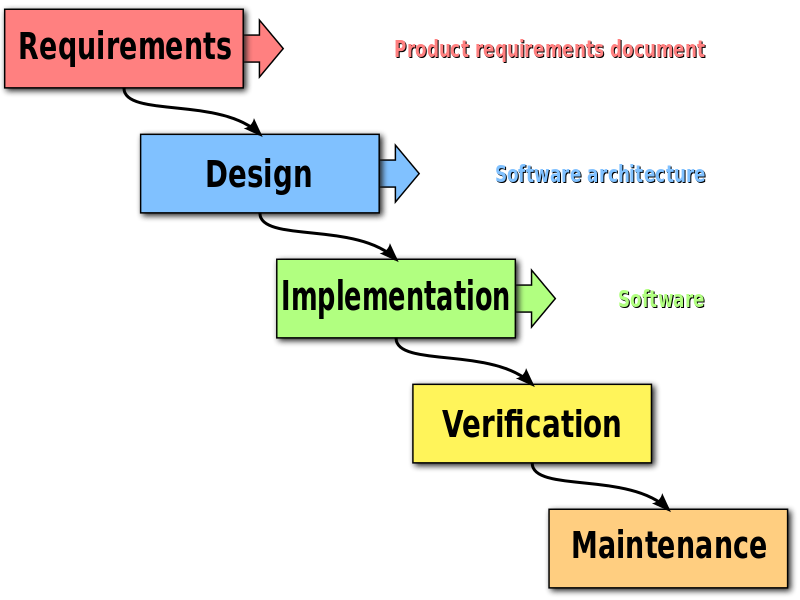
\includegraphics{images/image05.png}}

{On the contrary agile approaches are based on iterative and incremental
development, which means that the life cycles get passed through several
times. Thus agile approaches more often result in intermediate software
releases which encourage adaptations even late in the project's
development phase. Extreme programming is just one of many realisations
of agile software development methodologies. Since key aspects of its
definition are used in the implementation of the OBD software its
background as well as its approach are covered in this section. }

{The following sections layout the the reasons for choosing a particular
software development technique instead of deciding for another. In
addition to that the basics will be explained in particular together
with our approach and a final summarization containing our experiences
and knowledge we gathered by practicing those methodologies over the
course of the bachelor thesis.}

\hypertarget{h.qmc1u1ly9e76}{\subsection{\texorpdfstring{{Basics}}{Basics}}\label{h.qmc1u1ly9e76}}

{The}{~motivation}{~to apply }{the extreme programming methodology is
based on the already gathered know-how in this field by attending and
finishing the course ``Softwareentwicklung und Wissensmanagement'' in a
prior semester. }{Additionally, taking into consideration that the
software is designed to be used in an automotive context, the Automotive
SPICE standard, which is derived from the ISO 15504, has to be combined
with the test-driven development aspect of extreme programming.}

{Last but not least}{~prioritizing }{a consistent coding style within
the project to keep the source code itself as well as the overall
structure as clear as possible is intended. Thus simplifying future
maintenance and refactoring for programmers who are not implicitly the
initial developers of the source code. Furthermore this goal is pursue
this by basically agreeing to an internal coding standard based on the
book ``}{Clean Code: A Handbook of Agile Software Craftsmanship 1st
Edition}{'' by Robert C. Martin.}

\hypertarget{h.al3idr34x902}{\subsubsection{\texorpdfstring{{Extreme
Programming}}{Extreme Programming}}\label{h.al3idr34x902}}

{As mentioned}{~in the previous chapter the extreme programming attempt
is a type of agile software development. Generally it is desig}{ned to
enable small teams to develop software whose requirements change
frequently due to their ambiguous definition. Furthermore it is meant to
be a test-driven development approach. In other words a central point of
extreme programming is to write unit tests before any ``real'' code is
written. Thus securing the passing of newly written tests as well as
already implemented ones is very important. Rather than focussing on
testing each unit separately, extreme programming also requires to test
the whole system, in the best case, several times a day.}

{Best practice in extreme programming is to perform pair programming,
whereas in other software development techniques each developer has an
own task which needs to be merged in the end. Pair programming is done
by two programmers sitting in front of one PC using just one set of all
required peripherals (screen, keyboard, mouse etc.). Moreover it is
usual that the source code and design of the software gets refactored
and improved during the whole process for the purpose of keeping
flexibility high and complexity low.}

{Compared to other software development techniques there are some major
differences: First and foremost there is no specialization of the
developers on a single task, meaning that an extreme programming
programmer has to acquire}{~}{knowledge and new ways of thinking in all
parts which are related to software development. Starting with analysing
requirements over designing the software architecture to programming,
testing and maintaining the product after each release.}

{It should be emphasized that analyzing, designing, as well as the
developing of infrastructure and frameworks should }{not }{be performed
}{up-front}{. Extreme programming takes the view that those steps are
done when needed. This leads to a quicker development start as well as
more qualified decisions, due to gathered experience while dealing with
the project. Thus simplifying the estimate of which details deserve more
attention than others.}

{Another advice by Kent Beck in
{[}}{\href{https://www.google.com/url?q=http://dl.acm.org/citation.cfm?id\%3D318762\&sa=D\&ust=1460827923722000\&usg=AFQjCNHr2LQlB2UPss1lgCYPUbVINIAJOw}{http://dl.acm.org/citation.cfm?id=318762}}{{]}
}{is to communicate face-to-face or through efficient tests and clear
code rather than focussing on writing implementation documentation and
wasting time with maintaining those documents.}

\hypertarget{h.98eiyanf314e}{\subsubsection{\texorpdfstring{{Automotive
SPICE }}{Automotive SPICE }}\label{h.98eiyanf314e}}

{Automotive SPICE is a standard used to assess development processes of
control units in the automotive industry. It is derived from the ISO/IEC
15504, which is the general SPICE standard, whose main goal is the
assessment of processes in software development. SPICE is an
abbreviation for }{S}{oftware }{P}{rocess }{I}{mprovement and
}{C}{apability d}{E}{termination, which already clarifies the principal
aims. Automotive SPICE was developed by ~the AUTOSIG - the
}{Auto}{motive }{S}{pecial }{I}{nterest }{G}{roup, to whom many well
known manufacturers belong to, such as Audi, BMW, Fiat, Jaguar and a few
more.}

{Generally the Automotive SPICE Process Assessment Model (PAM) can be
described as a two-dimensional model consisting of a process dimension
and a capability dimension. The process dimension defines several
process categories, where processes are grouped depending on their type
of activity. The capability dimension is composed of capability levels,
which contain sets of process attributes who provide the measurable
characteristics of process capability.}

{The process dimension is described by the Automotive SPICE Process
Reference Model (PRM). Thereby 3 process categories are defined: Primary
life cycle processes, organizational life cycle processes and supporting
life cycle processes. Each category is furthermore divided into process
groups.}

{The primary life cycle processes category entails an acquisition
process group (ACQ), a supply process group (SPL) and an engineering
process group (ENG). Each group is then described by several processes
in detail. ACQ processes are used by the customer as well as the
supplier in order to acquire a product or a service. SPL processes are
meant for the supplier to actually supply a product or a service. ENG
processes cover the handling of customer's requirements defined in the
ACQ process as well as the specification, implementation and maintaining
of the software product and its relation to the system.}

{The supporting life cycle processes category consists only of one
support process group (SUP) whose processes can be employed by the other
processes at any time.}

{Lastly the organizational life cycle processes category includes a
management process group (MAN), a process improvement process group
(PIM) and a reuse process group (REU). MAN processes describe practices
to manage projects or processes. PIM processes deal with defining,
deploying and improving processes. REU processes systematically exploit
reuse opportunities in organization's reuse programs.}

\textsuperscript{\protect\hyperlink{ftnt16}{{[}16{]}}}

{The capability dimension describes six capability levels as following:}

\begin{itemize}
\tightlist
\item
  {Level 0 - Incomplete process:}
\end{itemize}

\begin{itemize}
\tightlist
\item
  {Process is not implemented or fails to achieve its purpose. At this
  level there is little or no evidence of any systematic achievement of
  the process purpose.}
\end{itemize}

\begin{itemize}
\tightlist
\item
  {Level 1 - Performed process:}
\end{itemize}

\begin{itemize}
\tightlist
\item
  {The implemented process achieves its process purpose.}
\end{itemize}

\begin{itemize}
\tightlist
\item
  {Level 2 - Managed process:}
\end{itemize}

\begin{itemize}
\tightlist
\item
  {The previously described performed process is now implemented in a
  managed fashion (planned, monitored and adjusted) and its work
  products are appropriately established, controlled and maintained.}
\end{itemize}

\begin{itemize}
\tightlist
\item
  {Level 3 - Established process:}
\end{itemize}

\begin{itemize}
\tightlist
\item
  {The previously described managed process is now implemented using a
  defined process that is capable of achieving its process outcomes.}
\end{itemize}

\begin{itemize}
\tightlist
\item
  {Level 4 - Predictable process:}
\end{itemize}

\begin{itemize}
\tightlist
\item
  {The previously described established process now operates within
  defined limits to achieve its process outcomes.}
\end{itemize}

\begin{itemize}
\tightlist
\item
  {Level 5 - Optimizing process:}
\end{itemize}

\begin{itemize}
\tightlist
\item
  {The previously described predictable process is continuously improved
  to meet relevant current and projected business goals.}
\end{itemize}

\hypertarget{h.mifm7q3zf07v}{\subsubsection{\texorpdfstring{{Clean
Code}}{Clean Code}}\label{h.mifm7q3zf07v}}

{Clean code cannot directly be considered as a software development
technique by itself. It is rather a common guideline for the whole
software development process. According to this, a programmer, who is
facing the task of developing new software, should prioritize on
producing clean code from the beginning rather than valuing speed and
coding sloppily.}

{Referring to {[}CLEAN CODE BUCH{]} there is no unique definition of
clean code. It is more likely that every programmer has his own point of
view when it comes to this question. Thus there are several definitions
which overlap partly as well as other ones which diverge widely. An
appropriate definition of clean code is coherent code, which is
characterized by making sense to a non familiar reader in a short period
of time. The reader should not be forced to put too much effort into
trying to decrypt the intention behind the code. Clean code also offers
some advantages. Source code which is written clean is rather likely to
be more stable. In addition to that maintaining clean code is basically
much more efficient when it comes to expanding or debugging.}

{Besides code conventions and design patterns which are depending on an
agreement}{~within a software developing team there is a set of rules
whic}{h can be followed to enhance the readability of the code according
to Robert C. Martin.}

{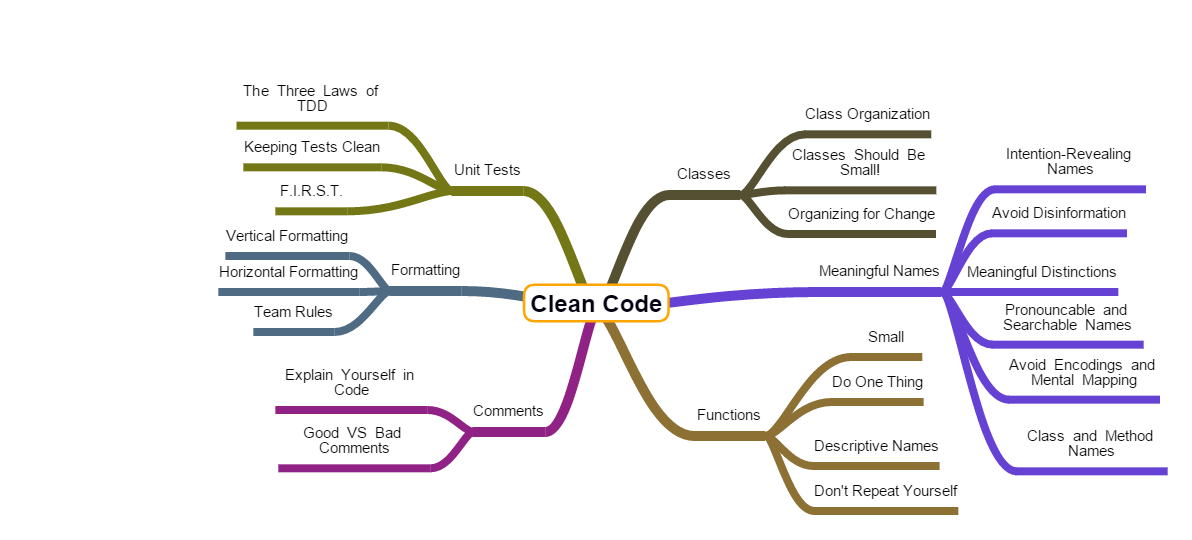
\includegraphics{images/image09.png}}

{The image above visualizes the clean code concepts by Robert C. Martin
based on ``Clean Code - A Handbook of Agile Software Craftsmanship''
which is considered to be among the most important concerning this
project. The shown mind map reveals a lot information about the basic
idea behind clean code according to Robert C. Martin. The following
paragraphs are describing each clean code feature a little more detailed
including some examples to clarify its intention.}

{Starting with }{meaningful names}{, intention-revealing names should
have a high priority, as the name of a function, class or variable
should be self-explaining, thus descriptive comments are considered
needless. The names should furthermore be changed, if a better one can
be found, e.g. a variable should rather be called
timeSinceFirstExecution than just single letters or abbreviations as x,
y, or tsfe. This also directly covers the subitems }{avoid
disinformation, meaningful distinctions, pronounceable and searchable
names}{. An example for bad naming would be the usage of uppercase ``o''
or lowercase ``L'' due to their similarity with ``0'' and ``1''.
Furthermore the author recommends class names consisting of nouns and
methods using verbs for naming.}

{It is advised to keep functions as small as possible, meaning that a
function consists only of a few lines without being in need of complex
nested structures, making them more readable and understandable. In
addition to that functions should only do one thing, but that they
should do well and not care for anything else. As highlighted in the
earlier paragraph function names should describe the purpose of the
function as detailed as possible, in such a way that no questions remain
open. If several lines of code are repeated over and over again
throughout the whole program it is better to encapsulate them into a
separate function, whereby unnecessary ~code duplication is avoided.}

{As phrased by Robert C. Martin in his book, clean code should
preferably contain as few comments as possible because comments are
mostly used to describe parts which are complicated and unorganized.
Further than that comments are considered as a sign for a programmer's
laziness, rather placing a comment than investing some time in
rethinking the naming of variables or functions. Nevertheless comments
which are considered good exist as well. Examples of such comments can
be looked up in ``Clean Code - A Handbook of Agile Software
Craftsmanship'' as well as examples which kind of comments should be
avoided.}

{Executing code formatting is also part of the clean code philosophy,
thus enhancing the general readability of the code as well as
simplifying it for future maintenance. There are some recommendations
for both vertical and horizontal formatting, as for instance splitting
concepts in such a way that closely associated code parts are vertically
dense. Same goes for the horizontal formatting, where a certain spacing
hints at relations and separations. Furthermore indentations should be
used to hierarchically separate different scopes.}

{Due to our extreme programming approach, the chapter ``Unit Tests''
attracted our attention as the software developing is built upon unit
testing and test driven development. There is a set of three rules
concerning test-driven development besides the already mentioned
priority of writing and executing tests before code is actually
implemented. The first rule says : ``You may not write production code
until you have written a failing unit test''. Rule number two is: ``You
may not write more of a unit test than is sufficient to fail, and not
compiling is failing''. The last rule amounts to: ``You may not write
more production code than is sufficient to pass the currently failing
test.''. The author recommends to pay attention to maintain the tests
clean as well, just as the code which is written afterwards to pass the
tests. Clean tests should be designed in such a manner that they obey
the ``F.I.R.S.T.'' principle, which is an acronym of five rules:}

{First of all tests should be }{f}{ast, meaning they run quickly so they
get executed frequently. Moreover test shall be }{i}{ndependent from
other tests as well as }{r}{epeatable in any environment. Another
characteristic is a boolean output, whether a test passes or fails, thus
}{s}{elf-validation is preferred over confusing log files or other means
of output. Lastly tests should be }{t}{imely, thus writing a test takes
place just right before writing the real code, due to the probability of
developing untestable code otherwise.}

{At long last c}{lasses are treated principally the same way as
functions, therefore they also should be as small as possible. As
opposed to functions the shortness is not measured in lines of code, it
is rather depending on the responsibilities of a class. This is covered
in the so called single responsibility principle. It purports that
classes or modules should have only one reason to change. Additionally
classes should be organized in such a way that they have an obvious
structure and is prepared in such a way that code changes do not ~crash
the program or induce complicated workarounds.}

{TBD}\textsuperscript{\protect\hyperlink{cmnt18}{{[}r{]}}}{~}

\hypertarget{h.8nawqkcgevsc}{\subsection{\texorpdfstring{{Realization}\textsuperscript{\protect\hyperlink{cmnt19}{{[}s{]}}}}{Realization{[}s{]}}}\label{h.8nawqkcgevsc}}

{The scientific aspect of this bachelor thesis is focused on the
combination of agile software development in the automotive context. The
foundation of this approach builds the Automotive SPICE PAM (PRM) model
as well as elements from Kent Beck's ``}{Extreme Programming
Explained}{''. This chapter will describe the design of combining these
software development processes, techniques and tools, which restrictions
were made and which compromises. The following chapter
}{\protect\hyperlink{h.ox6tol8shjj5}{Conclusion}}{~is then a subjective
summary of our experiences and insights.}

{The chosen software is in the vicinity of automotive software
development but still for users with little to no knowledge about the
structure and/or the automotive structure itself. Automotive software
development falls into the category of safety-critical systems, which
have high security and low fault tolerance criteria as well as strict
and complex testing of its software with severe consequences of
failure.}{~However safety uncritical systems, like average software,
}{have their focus on usability and visual representation as well as
extendability and effectiveness. Since this software belongs to two
areas of software development, ~the conclusion lies near that the
development techniques from both areas have valid ground for
application. Therefore it was necessary to design the development
process itself. Starting with the ACQ processes from the SPICE
development technique set, customer/system requirements were defined.}

{}

\begin{center}\rule{0.5\linewidth}{\linethickness}\end{center}

{}

{}

\href{}{}\href{}{}

\begin{longtable}[]{@{}ll@{}}
\toprule
\begin{minipage}[t]{0.47\columnwidth}\raggedright\strut
{Module}
\strut\end{minipage} &
\begin{minipage}[t]{0.47\columnwidth}\raggedright\strut
{We want an OBD tool\ldots{}}
\strut\end{minipage}\tabularnewline
\begin{minipage}[t]{0.47\columnwidth}\raggedright\strut
{1}
\strut\end{minipage} &
\begin{minipage}[t]{0.47\columnwidth}\raggedright\strut
{that is free of charge.}
\strut\end{minipage}\tabularnewline
\begin{minipage}[t]{0.47\columnwidth}\raggedright\strut
{2}
\strut\end{minipage} &
\begin{minipage}[t]{0.47\columnwidth}\raggedright\strut
{whose source code is available.}
\strut\end{minipage}\tabularnewline
\begin{minipage}[t]{0.47\columnwidth}\raggedright\strut
{3}
\strut\end{minipage} &
\begin{minipage}[t]{0.47\columnwidth}\raggedright\strut
{which can read and reset DTCs.}
\strut\end{minipage}\tabularnewline
\begin{minipage}[t]{0.47\columnwidth}\raggedright\strut
{4}
\strut\end{minipage} &
\begin{minipage}[t]{0.47\columnwidth}\raggedright\strut
{with which we can see online sensordata.}
\strut\end{minipage}\tabularnewline
\begin{minipage}[t]{0.47\columnwidth}\raggedright\strut
{5}
\strut\end{minipage} &
\begin{minipage}[t]{0.47\columnwidth}\raggedright\strut
{which is usable through USB interface.}
\strut\end{minipage}\tabularnewline
\begin{minipage}[t]{0.47\columnwidth}\raggedright\strut
{6}
\strut\end{minipage} &
\begin{minipage}[t]{0.47\columnwidth}\raggedright\strut
{whose usability is adapted to the target group.}
\strut\end{minipage}\tabularnewline
\begin{minipage}[t]{0.47\columnwidth}\raggedright\strut
{7}
\strut\end{minipage} &
\begin{minipage}[t]{0.47\columnwidth}\raggedright\strut
{which is easily extendable.}
\strut\end{minipage}\tabularnewline
\begin{minipage}[t]{0.47\columnwidth}\raggedright\strut
{8}
\strut\end{minipage} &
\begin{minipage}[t]{0.47\columnwidth}\raggedright\strut
{which conforms the WWH-OBD and European OBD standards.}
\strut\end{minipage}\tabularnewline
\begin{minipage}[t]{0.47\columnwidth}\raggedright\strut
{9}
\strut\end{minipage} &
\begin{minipage}[t]{0.47\columnwidth}\raggedright\strut
{which is usable with a range of OBD-HW or easily extendable to third
party hardware.}
\strut\end{minipage}\tabularnewline
\begin{minipage}[t]{0.47\columnwidth}\raggedright\strut
{10}
\strut\end{minipage} &
\begin{minipage}[t]{0.47\columnwidth}\raggedright\strut
{which can be tested without any hardware.}
\strut\end{minipage}\tabularnewline
\bottomrule
\end{longtable}

{}

{The next step according to SPICE is to parse those customer
requirements to software and hardware requirements. The latter are
simple, since this project only requires an average ELM327. The software
requirements, on the other hand, were designed quite thoroughly. }

{}

\begin{center}\rule{0.5\linewidth}{\linethickness}\end{center}

{}

{}

{}

{LEFT BLANK FOR FUNCTIONAL
REQUIREMENTS----------------------------------}

{(pdf in landscape pages)}

\begin{center}\rule{0.5\linewidth}{\linethickness}\end{center}

{}

{}

{The detailed design, which would be the next task, resulted in the
first compromis. It seemed smart to move the detailed design of each
package to right before implementing it. This corresponds to agile
software development requirement of doing the design of the task to
implement as late as possible.}

{The implementation of the packages was done by using the following
agile software development techniques:}

\begin{itemize}
\tightlist
\item
  {Test Driven Development}
\end{itemize}

\begin{itemize}
\tightlist
\item
  {trust into the produced code}
\end{itemize}

\begin{itemize}
\tightlist
\item
  {Pair Programming}
\end{itemize}

\begin{itemize}
\tightlist
\item
  {resulting in less time to search bugs}
\end{itemize}

\begin{itemize}
\tightlist
\item
  {Constant Refactoring}
\end{itemize}

\begin{itemize}
\tightlist
\item
  {resulting in code resistance and no functionality duplication}
\end{itemize}

{Since the rough design and thus the order in which the single
functionalities have to be implemented was already defined by the SPICE
processes, agile software development for the single packages could
easily be applied. Although this approach breaks the premise of agile
software development to have as little design overhead as possible, but
instead doing the design when implementing, it seems to be valid
compromise to merge the SPICE PRM with the techniques of agile software
development. }

{Summarized, the approach can be interpreted as the usable process
definitions of the SPICE PRM with its advantages, combined with the
freedom and scalability of agile software development. The difference to
the classic SPICE model is including the execution order of certain
processes, like detailed design. Furthermore the comparison to the
requirements is not tested at the completion of the project, but rather
defined before even beginning programming, through the unit tests. Agile
software development differs from its classical approach by taking some
flexibility through the division into packages at the ACQ phase of the
SPICE models. All in all the approach seems valid especially for this
kind of software and was tested out by implementing code in that certain
area as well. A further description of the gained insights can be found
in the next chapter. }

\hypertarget{h.xkuwr51j6zad}{\subsection{\texorpdfstring{{Conclusion}}{Conclusion}}\label{h.xkuwr51j6zad}}

{The combination of spontaneous agile software development with rigid
Automotive SPICE is fusing two contradictory software development areas.
This results in numerous issues and gathered experience which will be
shared in this chapter.}

{Right after the SPICE PRM planning phase was finished, the actual work
on the tools started. The first achievable goal was to establish a
running communication via the serial interface, more precisely
connecting over the USB interface. Due to the early stage of
development, more accurately the lack of practical experience with the
newly created methodology, the implementation took place without real
unit tests. Furthermore meaningful testing would have been complicated
as well, due to the necessity of implementing mocking classes to
successfully test all parts of the serial communication.}

{After completing the serial communication the development of the OBD
related parts were planned. The longer the focussing on the realization
of the already planned processes and detailed requirements of the OBD
control unit emulation software and the actual OBD tool lasted, many
overlaps arose. Thus leading to the decision of drifting off from the
existing plan and encapsulating the overlapping details in a so called
OBD middleware. Its purpose was to provide classes and functions which
are needed by both softwares.}

{As time went by we adjusted to the characteristics of }{agile software
development, meaning the writing of unit tests right before actual
production code was practiced constantly as well as regularly switching
the roles as suggested for pair programming. While one wrote an unit
test which failed after its immediate execution the other one had to
observe and point out possible issues. After the unit test was finished,
the developer of the unit test switched into the observer role and the
other one implemented a solution to pass the unit test as well as going
for the next unit test, alternating the roles constantly.}

{Over time the quality of the unit tests improved and furthermore the
exertion of pair programming led to less debugging and refactoring than
we were used to compared to previous non agile projects.}

{Besides the decision of developing a middleware for the OBD software
the basic principle of structuring retained as planned from the
beginning on. Unfortunately cuts in the final softwares were made due to
underestimating the time which was consumed by the general
implementation and refactoring.}

{}

{Hallo ende wo bist du?}

\hypertarget{h.mzh64o82gvdq}{\section{\texorpdfstring{{References}}{References}}\label{h.mzh64o82gvdq}}

{USB in a Nutshell}

{ELM Commands}

{OBD Commands}

{Florian Schäffer }

{Kent Beck}

{Robert C. Martin}

{Automotive SPICE}

{ISO 15031}

{}

\begin{center}\rule{0.5\linewidth}{\linethickness}\end{center}

\protect\hyperlink{ftntux5fref1}{{[}1{]}}{~http://www.amazon.de/iParaAiluRy-Interface-Diagnose-Auto-Scanner-Scan-Werkzeug/dp/B00ZZMX0GY/ref=sr\_1\_1?ie=UTF8\&qid=1456145102\&sr=8-1\&keywords=elm327+usb}

\protect\hyperlink{ftntux5fref2}{{[}2{]}}{~}{Koscher et al. Experimental
Security Analysis of a Modern Automobile. }{In Security and Privacy
(SP), 2010 IEEE Symposium on}{, 2010,
DOI:}{\href{https://www.google.com/url?q=http://dx.doi.org/10.1109/SP.2010.34\&sa=D\&ust=1460827923758000\&usg=AFQjCNGcRSFStl3xg5e6ejJJzzZ7UxIUnw}{~}}{\href{https://www.google.com/url?q=http://dx.doi.org/10.1109/SP.2010.34\&sa=D\&ust=1460827923759000\&usg=AFQjCNE4oc1RPHni0YpsJqyZNhOBWoP62A}{10.1109/SP.2010.34}}

\protect\hyperlink{ftntux5fref3}{{[}3{]}}{~vgl. USB in a Nutshell URL:
}{\href{https://www.google.com/url?q=http://www.beyondlogic.org/usbnutshell/usb4.shtml\&sa=D\&ust=1460827923757000\&usg=AFQjCNFllIVNcog2CsTPDWQSr9Zs2N-iww}{http://www.beyondlogic.org/usbnutshell/usb4.shtml}}{~Stand:
Feb. 2016}

\protect\hyperlink{ftntux5fref4}{{[}4{]}}{see URL:
}{\href{https://www.google.com/url?q=http://www.usb.org/developers/docs/\&sa=D\&ust=1460827923759000\&usg=AFQjCNHaPtIxFF98hmmxU-1fwdcMF5vqZA}{http://www.usb.org/developers/docs/}}{~Stand:
14.02.2016}

\protect\hyperlink{ftntux5fref5}{{[}5{]}}{~http://www.libusb.org/}

\protect\hyperlink{ftntux5fref6}{{[}6{]}}{~http://man7.org/linux/man-pages/man3/termios.3.html}

\protect\hyperlink{ftntux5fref7}{{[}7{]}}{~https://sourceforge.net/projects/usb-vhci/}

\protect\hyperlink{ftntux5fref8}{{[}8{]}}{~http://www.usb.org/developers/docs/}

\protect\hyperlink{ftntux5fref9}{{[}9{]}}{~https://dev.mysql.com/downloads/connector/cpp/}

\protect\hyperlink{ftntux5fref10}{{[}10{]}}{~http://elmelectronics.com/ELM327/AT\_Commands.pdf}

\protect\hyperlink{ftntux5fref11}{{[}11{]}}{~http://libxmlplusplus.sourceforge.net/reference/html/index.html}

\protect\hyperlink{ftntux5fref12}{{[}12{]}}{~}{\href{https://www.google.com/url?q=https://sourceforge.net/projects/usb-vhci/\&sa=D\&ust=1460827923761000\&usg=AFQjCNEYf3zs9zmQHnlPkVsLeqw4mINQYQ}{https://sourceforge.net/projects/usb-vhci/}}{~stand
22.02.2016}

\protect\hyperlink{ftntux5fref13}{{[}13{]}}{~}{\href{https://www.google.com/url?q=http://linux.die.net/man/8/insmod\&sa=D\&ust=1460827923761000\&usg=AFQjCNGeB1IWdK3zghqXBgFULixNgKXhJw}{http://linux.die.net/man/8/insmod}}{~stand
22.02.2016}

\protect\hyperlink{ftntux5fref14}{{[}14{]}}{~https://sourceforge.net/projects/usb-vhci/files/?source=navbar}

\protect\hyperlink{ftntux5fref15}{{[}15{]}}{~https://sourceforge.net/projects/usb-vhci/files/?source=navbar}

\protect\hyperlink{ftntux5fref16}{{[}16{]}}{~vgl. link zum spice
document}

\protect\hyperlink{cmntux5fref1}{{[}a{]}}{Write abstract}

\protect\hyperlink{cmntux5fref2}{{[}b{]}}{klingt komisch, vielleicht
``planned''?}

\protect\hyperlink{cmntux5fref3}{{[}c{]}}{Add Chapter references}

\protect\hyperlink{cmntux5fref4}{{[}d{]}}{den satz versteh ich leider
gar nicht :( wenn das für techniker sinn macht dann lassts ihn stehn,
ansonsten würde ich umschreiben}

\protect\hyperlink{cmntux5fref5}{{[}e{]}}{security chapter?}

\protect\hyperlink{cmntux5fref6}{{[}f{]}}{USB, Can erwähnen (not
covered), K-Line for obdcodes communication}

\protect\hyperlink{cmntux5fref7}{{[}g{]}}{besser vielleicht ``part''?}

\protect\hyperlink{cmntux5fref8}{{[}h{]}}{Find refernece other than
wikipedia}

\protect\hyperlink{cmntux5fref9}{{[}i{]}}{packages?}

\protect\hyperlink{cmntux5fref10}{{[}j{]}}{der vollständigkeit halber
alle anführen?}

\protect\hyperlink{cmntux5fref11}{{[}k{]}}{Threading in serial
communication}

\protect\hyperlink{cmntux5fref12}{{[}l{]}}{dont forget}

\protect\hyperlink{cmntux5fref13}{{[}m{]}}{general approach + fill with
code examples and refactoring examples + class diagram + how was it
abstracted?}

\protect\hyperlink{cmntux5fref14}{{[}n{]}}{general approach + fill with
code examples and refactoring examples + class diagram + how was it
abstracted?}

\protect\hyperlink{cmntux5fref15}{{[}o{]}}{Short introduction merging
functionalities of middleware Problems , advantages, Gui, QT}

\protect\hyperlink{cmntux5fref16}{{[}p{]}}{what is it?}

{how to use it?}

{functionalties it represents from middlewarepackages}

\protect\hyperlink{cmntux5fref17}{{[}q{]}}{libvhci compilation and all
compiliations}

\protect\hyperlink{cmntux5fref18}{{[}r{]}}{Übergang auf nächstes
Kapitel?}

\protect\hyperlink{cmntux5fref19}{{[}s{]}}{system requirements structure
project structure as pictrues}
